% ─────────────────────────────────────────────────────────────────────────────
%  Chương 3 — Các kết quả đã đạt được
%  Hướng dẫn của Khoa: giới thiệu sản phẩm, giao diện, chức năng chính; nếu có
%  kết quả kiểm thử thì nêu test case, phân tích lỗi và cách khắc phục.
%
%  LƯU Ý: Các số liệu trong chương này đo trên máy Apple M4 / 24 GB, macOS 26.4,
%  PyTorch 2.13 chạy trên MPS, trọng số yolov8n. Chạy lại trên máy và dữ liệu
%  của bạn rồi cập nhật, đừng chép nguyên số.
% ─────────────────────────────────────────────────────────────────────────────
\chapter{Các kết quả đã đạt được}
\label{ch:ketqua}

\section{Sản phẩm bàn giao}
\label{sec:sanpham}

Sản phẩm là một ứng dụng web hoàn chỉnh gồm máy chủ xử lý ảnh và giao diện quản
trị, chạy được trên máy tính cá nhân không cần GPU rời. Mã nguồn chia hai thư mục
\code{backend/} và \code{frontend/}, kèm tài liệu cài đặt.

\begin{table}[H]
\centering
\caption{Quy mô mã nguồn theo thành phần.}
\label{tab:quymo}
\small
\begin{tabularx}{\textwidth}{@{}lXr@{}}
\toprule
\textbf{Thành phần} & \textbf{Nội dung} & \textbf{Số dòng} \\
\midrule
\code{backend/app/}  & Engine xử lý ảnh, REST API, truy cập cơ sở dữ liệu & 4.772 \\
\code{frontend/src/} & Giao diện React, TypeScript & 4.319 \\
\code{scripts/}      & Script đo thực nghiệm, kiểm thử và dựng hình minh hoạ & 1.006 \\
\code{report/}       & Mã nguồn LaTeX của báo cáo này & 2.820 \\
\midrule
\multicolumn{2}{@{}l}{\textbf{Tổng cộng}} & \textbf{12.917} \\
\bottomrule
\end{tabularx}
\end{table}

Số dòng đếm bằng \code{wc -l}, đã bao gồm chú thích và dòng trống.

Máy chủ cung cấp 38 điểm cuối API, chia thành năm nhóm: camera, pipeline, sự
kiện, xem lại và quản trị. Tài liệu API tự sinh theo chuẩn OpenAPI, truy cập tại
\code{/docs}.

Kèm theo mã nguồn là thư mục \code{output/} chứa video kết quả của từng pipeline
đếm, mỗi tệp đã in sẵn vạch đếm, hộp giới hạn và bảng số Vào/Ra lên khung hình.
Video sinh bằng \code{scripts/kiem\_thu\_dem.py}; tham số vạch lấy trực tiếp từ
API nên luôn khớp với cấu hình đang chạy trong hệ thống.

\begin{table}[H]
\centering
\caption{Video kết quả bàn giao. Mỗi tệp ứng với một pipeline, không phải một
video nguồn --- một camera chạy nhiều pipeline thì có nhiều tệp, nên tên tệp kèm
mã pipeline.}
\label{tab:videoout}
\small
\begin{tabularx}{\textwidth}{@{}Xllc@{}}
\toprule
\textbf{Pipeline} & \textbf{Vạch} & \textbf{Nguồn} & \textbf{Vào/Ra} \\
\midrule
Đếm người qua cửa hàng           & Ngang, lật & Cửa hàng tiện lợi & 1/0 \\
Đếm người qua cửa sảnh ga        & Ngang      & Cửa ra vào sảnh ga & 1/5 \\
Đếm qua vạch --- Cửa tàu điện    & Chéo       & Ga tàu điện ngầm & 6/10 \\
Đếm qua vạch --- người đeo túi   & Chéo, lật  & Ga tàu điện ngầm & 9/6 \\
Đếm người mặc áo trắng           & Dọc        & Cổng ra vào & 2/4 \\
Đếm người qua cổng               & Dọc        & Cổng ra vào & 2/4 \\
\bottomrule
\end{tabularx}
\end{table}

\section{Giao diện và chức năng chính}
\label{sec:chucnang}

\subsection{Trang giám sát}

\begin{figure}[H]
\centering
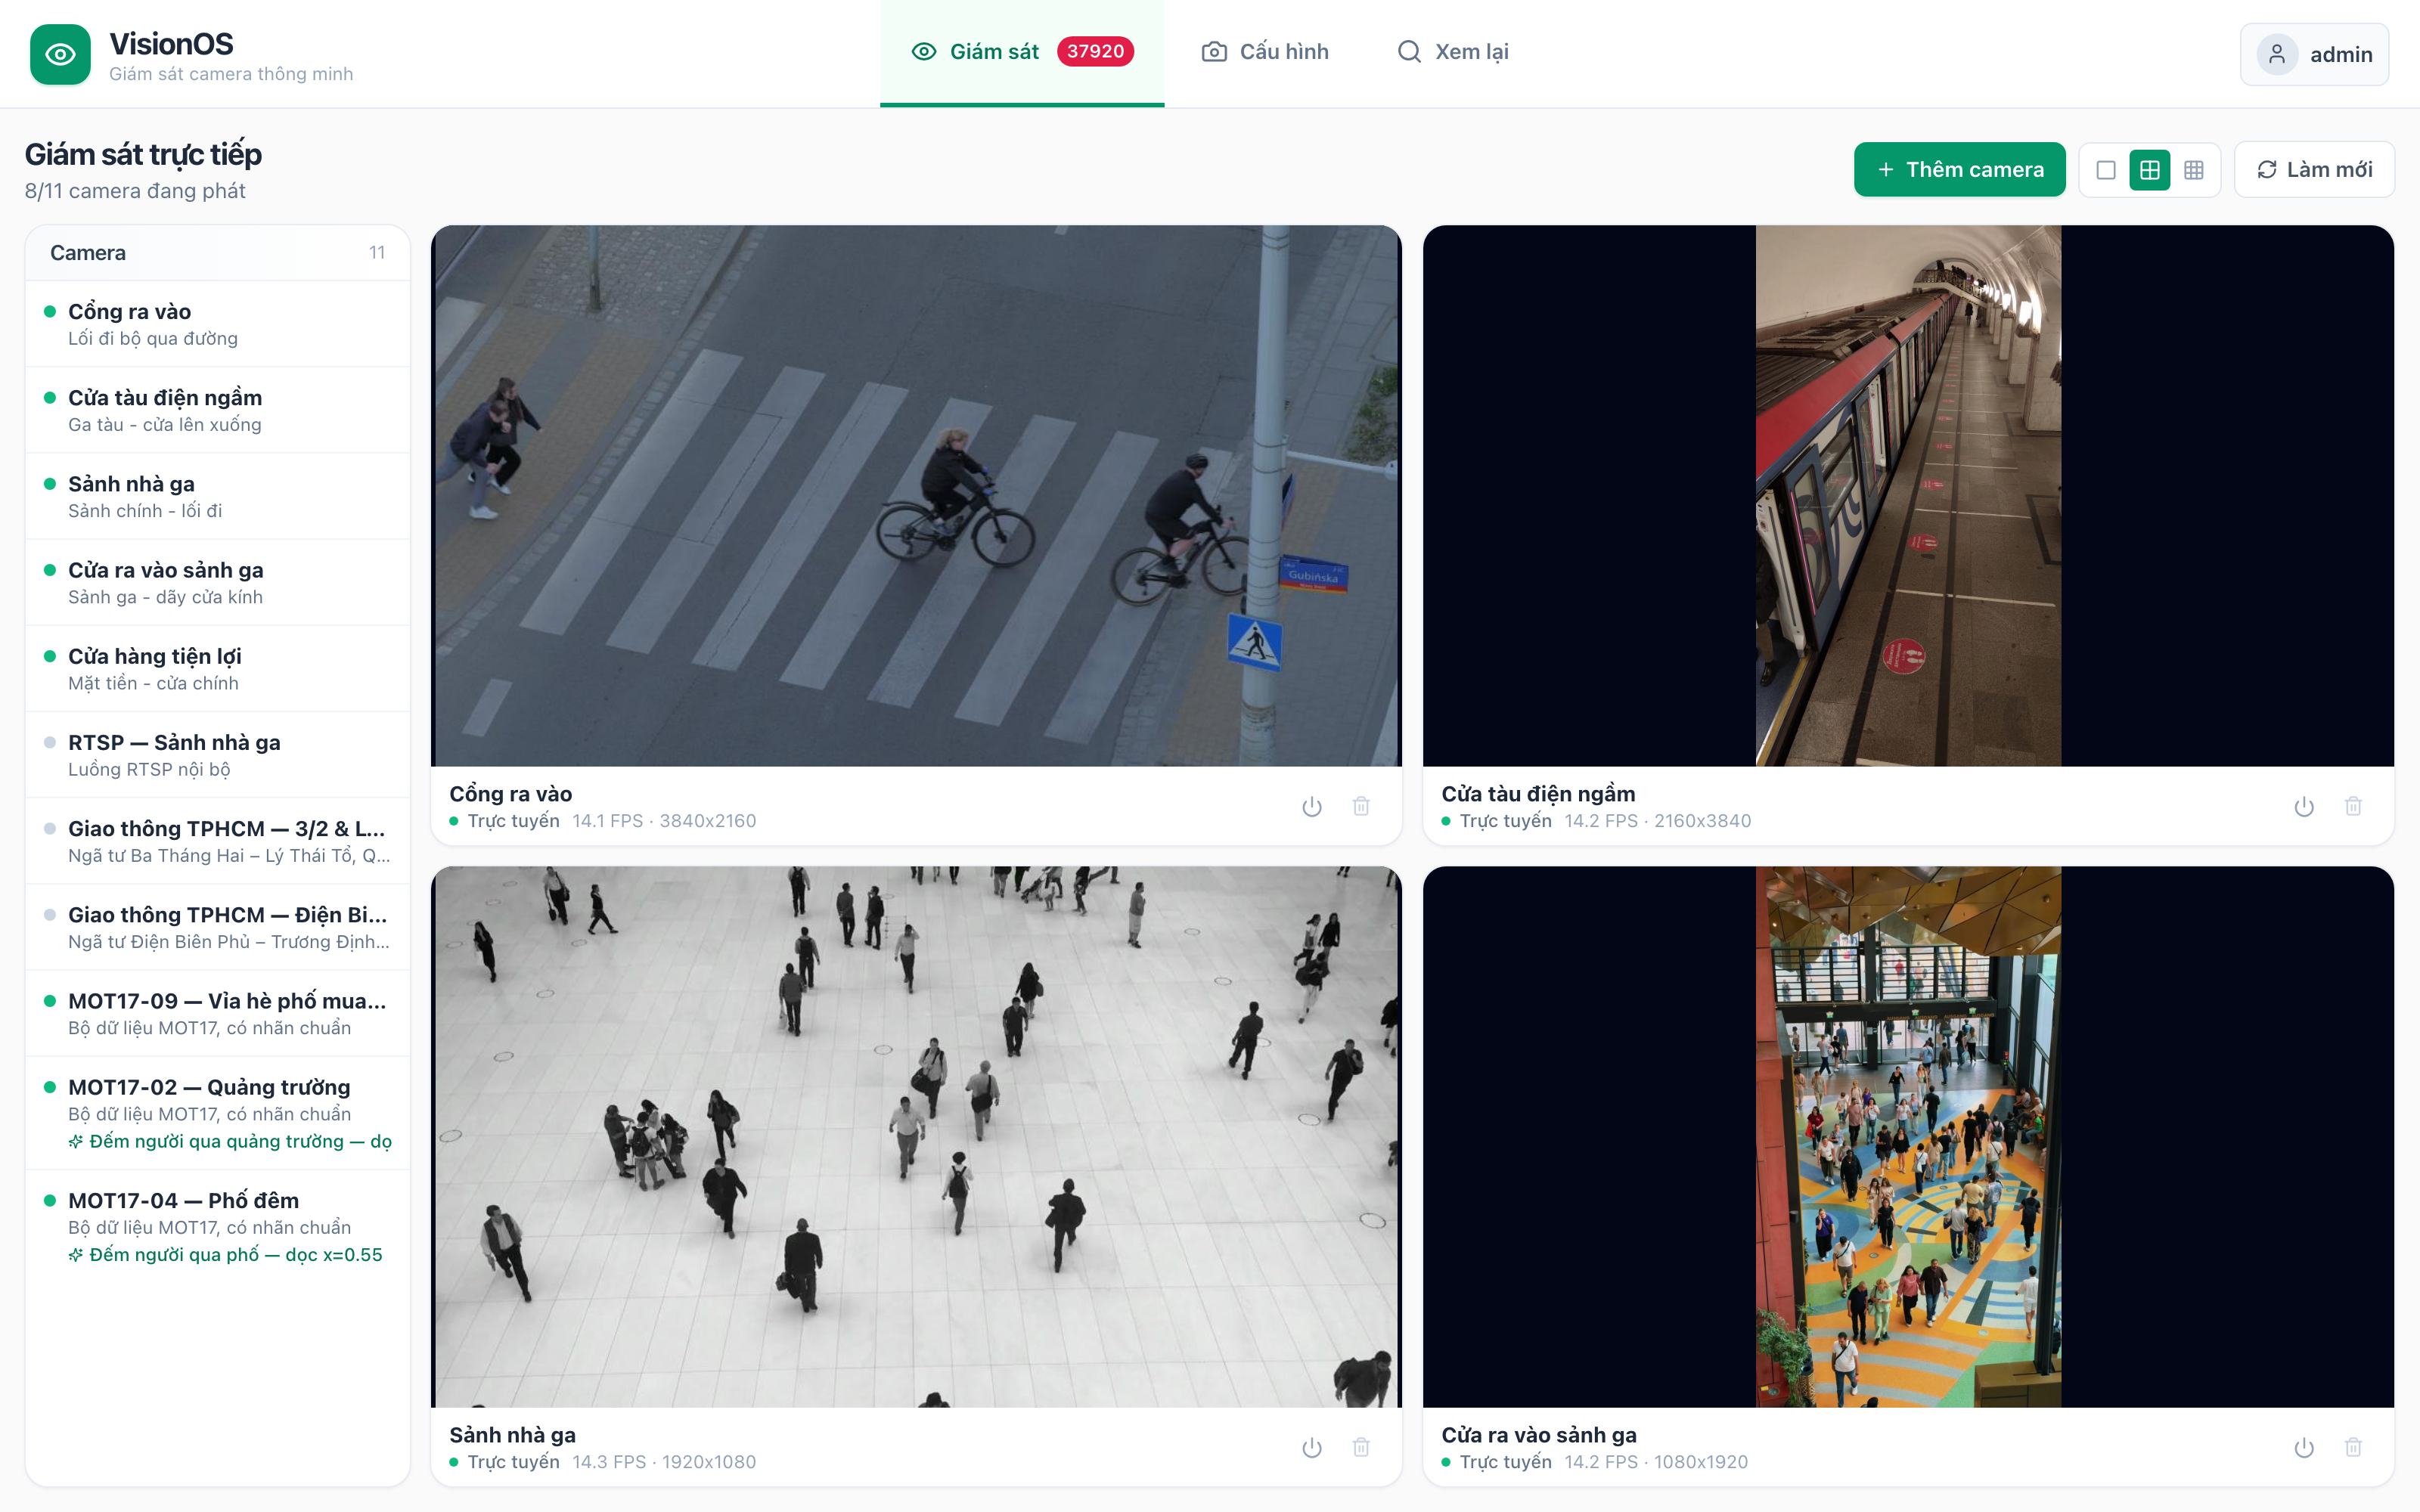
\includegraphics[width=\textwidth]{figures/ui_live.png}
\caption{Trang giám sát. Lưới tự co số cột theo số camera đang hiển thị nên khung
hình luôn lấp hết chiều ngang và chiều cao còn lại.}
\label{fig:ui-live}
\end{figure}

Lưới hiển thị chuyển được giữa ba mức 1$\times$1, 2$\times$2 và 3$\times$3. Mỗi ô
hiện tên camera, trạng thái kết nối, tốc độ xử lý và độ phân giải. Nút nguồn trên
từng ô cho phép ngắt luồng, khi đó ô chuyển sang màn hình chờ và hệ thống tự kết
nối lại theo chu kỳ ba giây.

\begin{figure}[H]
\centering
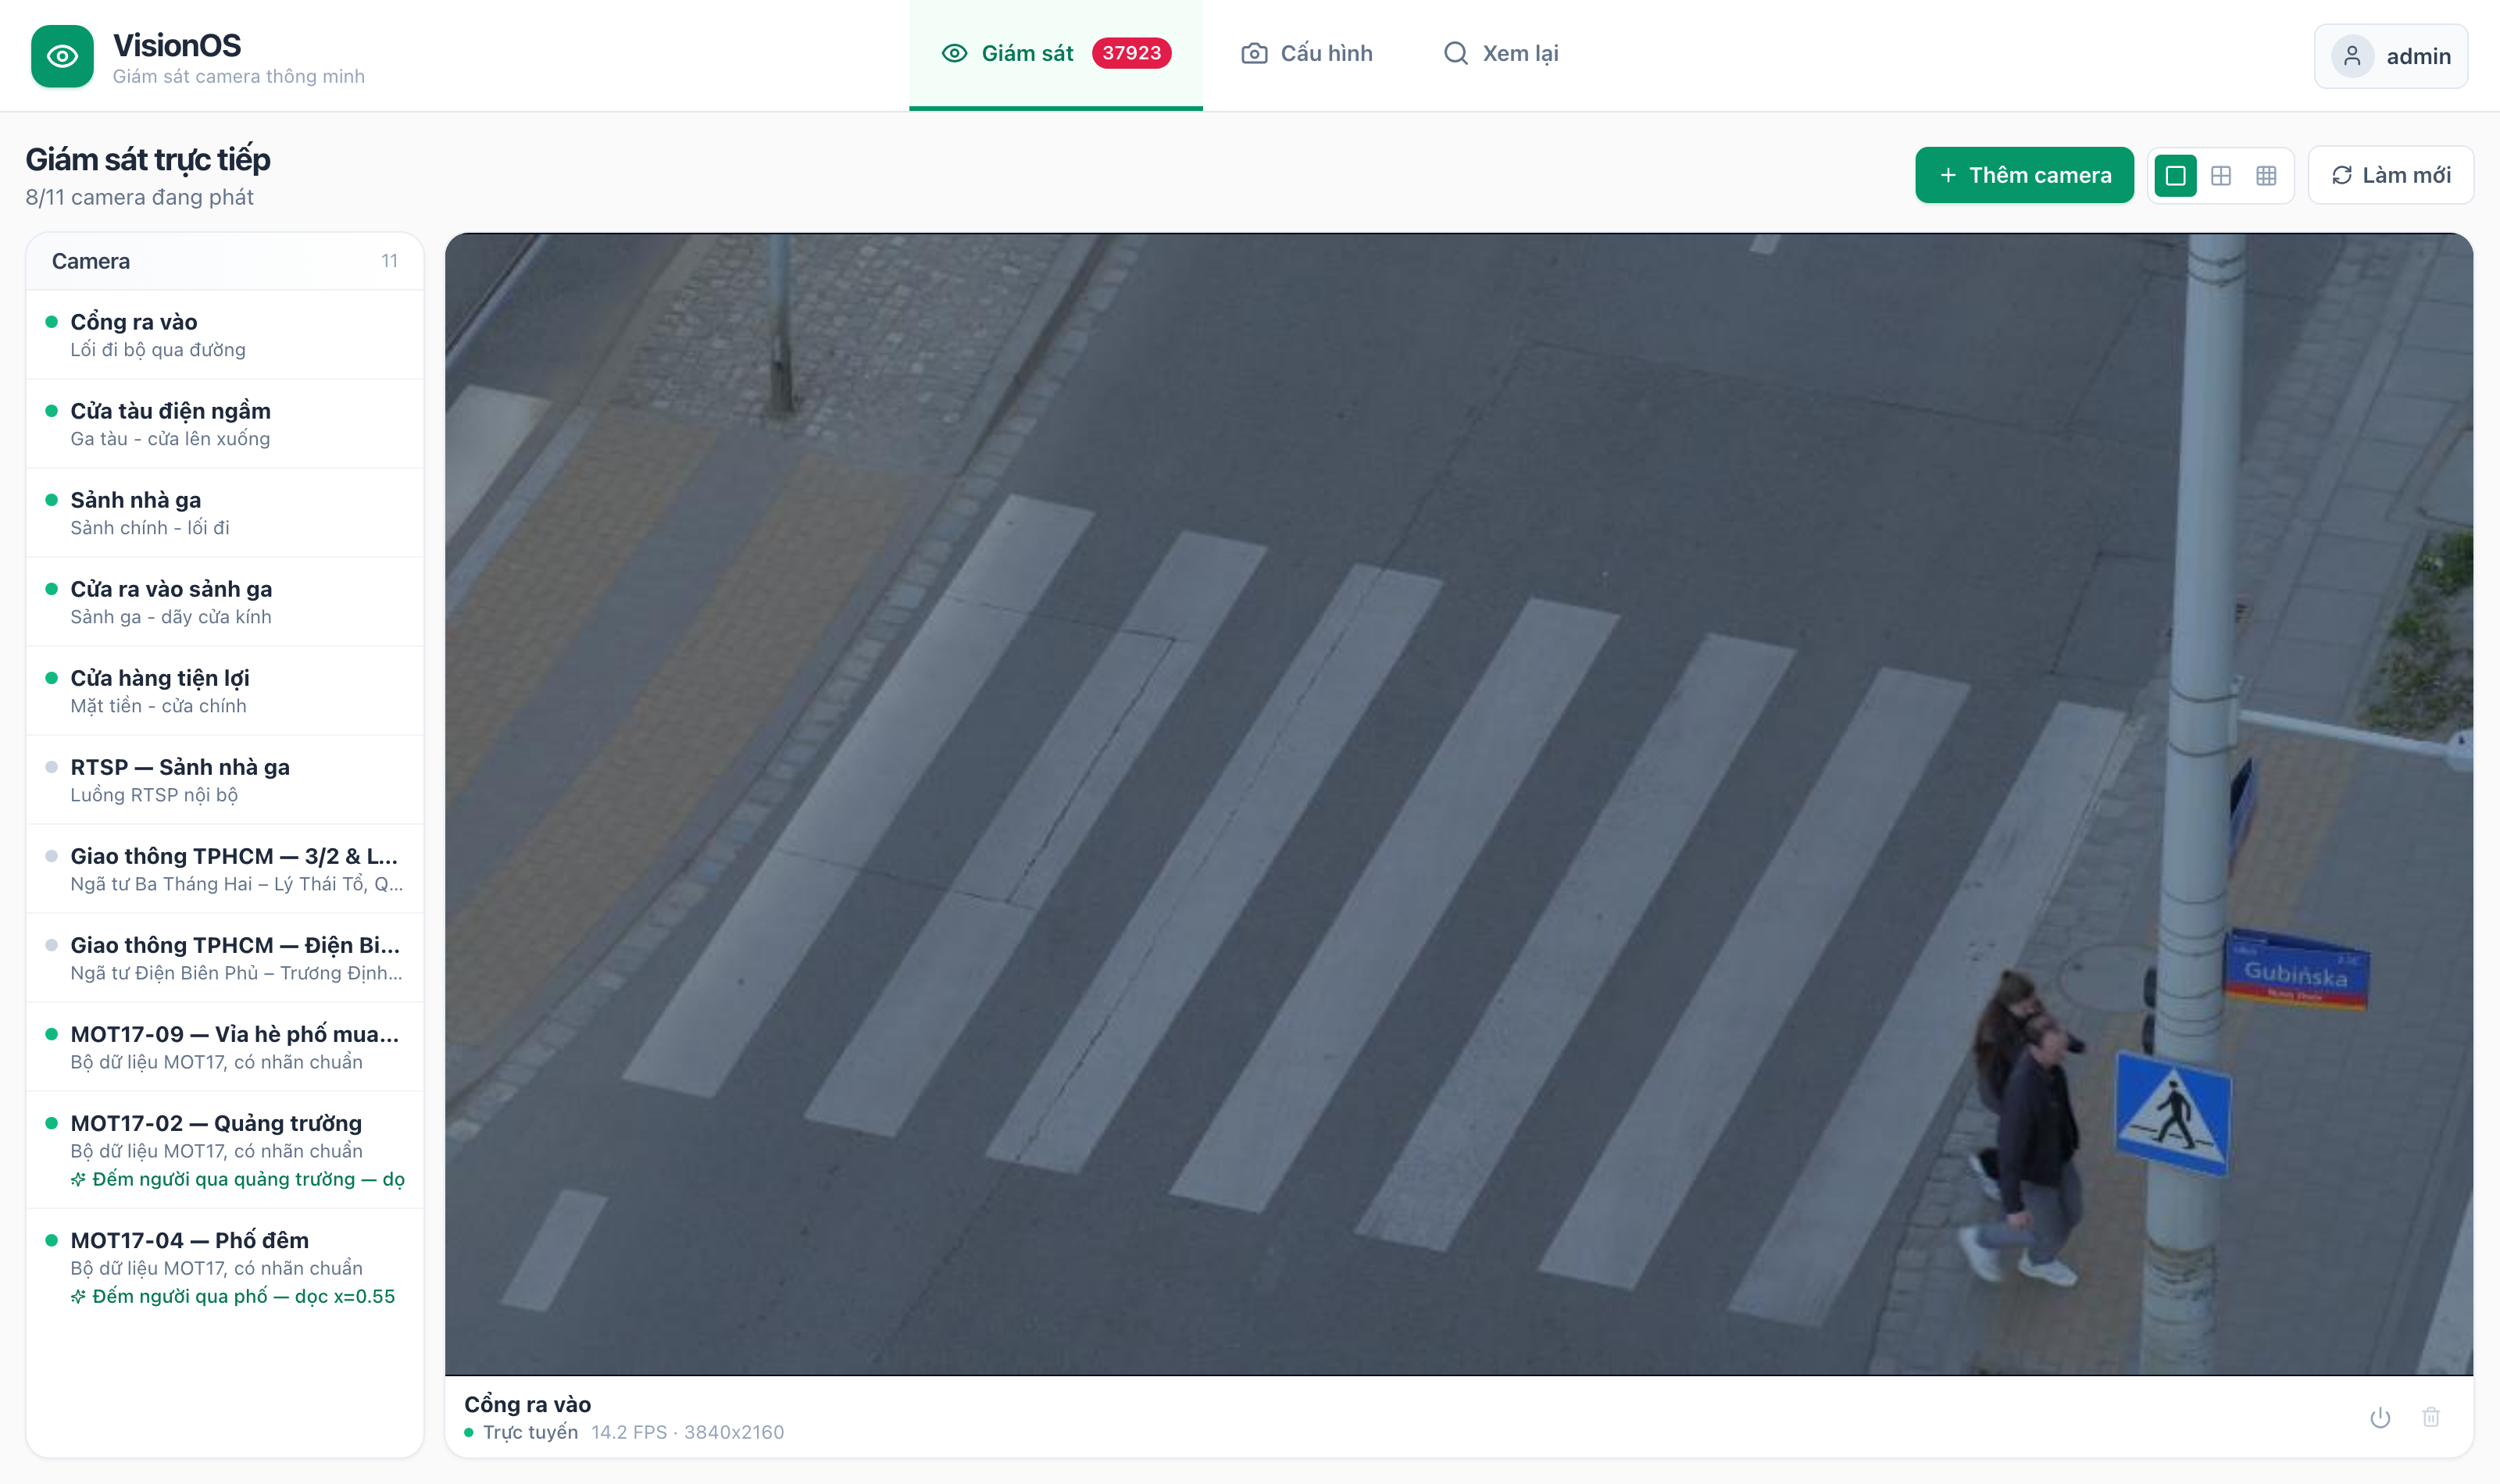
\includegraphics[width=\textwidth]{figures/ui_alert.png}
\caption{Cảnh báo chỉ hiện khi phóng to một camera đang chạy pipeline, và chỉ hiện
cảnh báo của đúng camera đó.}
\label{fig:ui-alert}
\end{figure}

Bảng cảnh báo làm mới bốn giây một lần. Mỗi sự kiện có hai nút: xác nhận chuyển
trạng thái sang \emph{đang xử lý}, đóng chuyển sang \emph{đã đóng} kèm thời điểm
xử lý.

Ảnh trong bảng cảnh báo chỉ rộng 200 điểm ảnh, đủ để biết có chuyện gì xảy ra
nhưng không đủ để nhận mặt người. Bấm vào ảnh sẽ mở bản 1280 điểm ảnh phủ kín màn
hình, đóng lại bằng phím \code{Esc}, bằng nút đóng, hoặc bằng cách bấm ra ngoài
khung. Cùng một thành phần giao diện được dùng lại ở trang xem lại, khác ở chỗ
tại đó có thêm nút nhảy tới đúng giây trong đoạn video --- ở màn giám sát trực
tiếp thì không có đoạn video tương ứng nên nút tự ẩn.

\subsection{Trang cấu hình}

\begin{figure}[H]
\centering
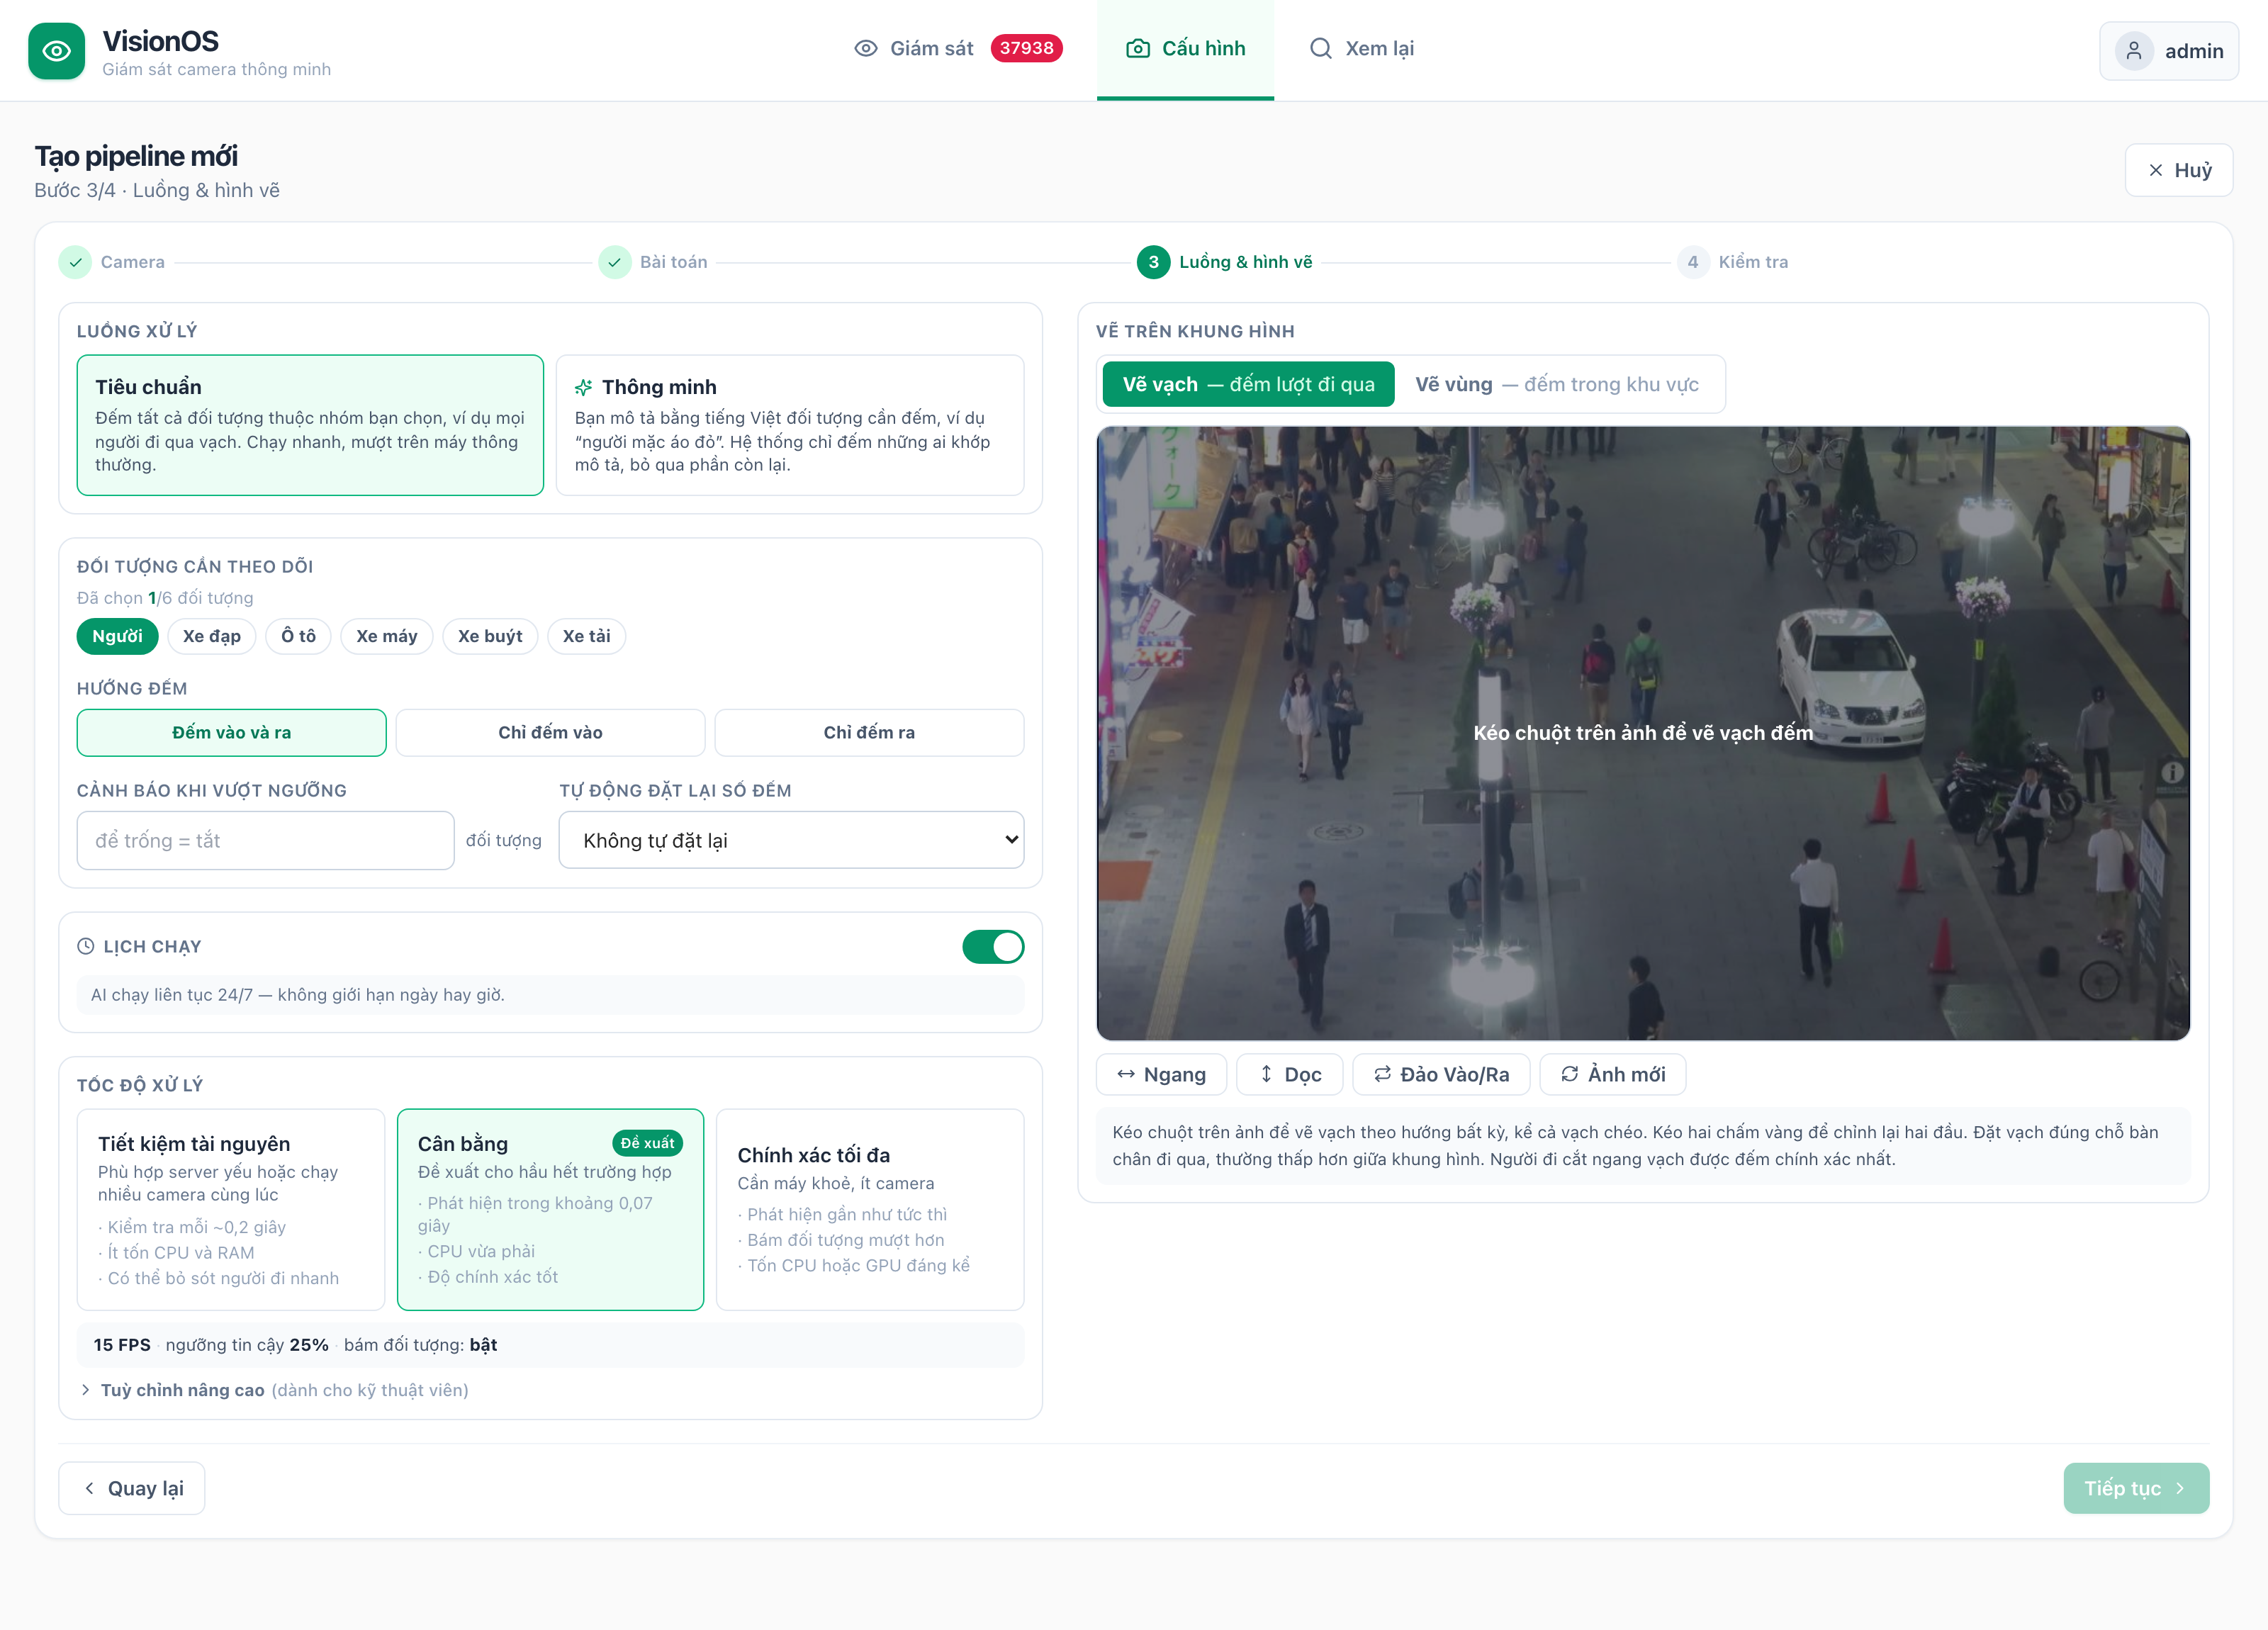
\includegraphics[width=\textwidth]{figures/ui_pipeline.png}
\caption{Bước vẽ vạch đếm. Hai mũi tên cho biết phía nào được tính là Vào trước
khi pipeline chạy, tránh phải chạy thử rồi mới phát hiện ngược chiều.}
\label{fig:ui-pipeline}
\end{figure}

Trình hướng dẫn bỏ qua bước vẽ vạch khi người dùng chọn bài toán nhận diện, vì
bài toán này không cần ranh giới. Pipeline đang chạy nhận cấu hình mới ngay khi
lưu, không phải tắt đi bật lại.

Bảng pipeline đã tạo liệt kê tên, camera, bài toán, chế độ và trạng thái. Nút
\emph{Sửa} mở lại chính trình hướng dẫn đó với dữ liệu đã điền sẵn, bắt đầu từ
bước chọn bài toán --- bước chọn camera bị khoá vì pipeline gắn chặt với camera
nó theo dõi, muốn đổi camera thì tạo pipeline mới. Sửa được cả vạch, vùng lẫn mọi
tham số, kể cả khi pipeline đang chạy.

\subsubsection*{Quan hệ nhiều--nhiều giữa camera và pipeline}
\label{sub:nhieu-pipeline}

Bản đầu chỉ cho mỗi camera chạy đúng một pipeline: hàm \code{attach\_pipeline}
chủ động tắt các pipeline khác của cùng camera. Ràng buộc này không hợp với nhu
cầu thực tế --- một camera cổng vừa cần đếm người qua cửa vừa cần đếm xe trong
bãi, hai bài toán khác nhau trên cùng khung hình.

Về phía chạy, mỗi pipeline cần bộ bám vết, bộ đếm, bộ lọc Thông minh và lịch chạy
riêng; dùng chung sẽ lẫn số đếm và lẫn mã định danh vết. Toàn bộ những thứ đó
được gom vào lớp \code{PipelineRuntime}, còn \code{CameraWorker} giữ một danh
sách các runtime thay vì một bộ biến đơn lẻ.

Điểm phải cân nhắc là chi phí GPU. Cách làm thẳng thừng --- mỗi pipeline tự gọi
YOLO một lần --- khiến ba pipeline tốn gấp ba lần suy luận, trong khi
mục~\ref{sub:mps-segfault} đã cho thấy GPU chính là nút thắt của hệ thống. Vì vậy
phần phát hiện được tách khỏi phần bám vết: vòng lặp gọi YOLO \emph{một lần} với
hợp các lớp cần tìm và ngưỡng tin cậy thấp nhất, rồi mỗi pipeline tự lọc lại theo
lớp và ngưỡng của riêng nó và tự bám vết. Chi phí GPU vì thế không tăng theo số
pipeline.

Ở màn giám sát, vẽ chồng kết quả của mọi pipeline lên một khung hình sẽ rối, nên
mỗi pipeline giữ bản vẽ riêng và ô camera có nút chuyển qua lại; luồng video nhận
thêm tham số \code{pipeline\_id}.

Chiều ngược lại --- một lần tạo cho nhiều camera --- không cần đổi lược đồ cơ sở
dữ liệu: trình hướng dẫn cho tick nhiều camera rồi sinh ra mỗi camera một pipeline
độc lập, cùng tham số nhưng số đếm tách bạch, tên ghép thêm tên camera cho khỏi
trùng. Riêng hình vẽ bắt buộc phải làm cho từng camera, vì vạch đặt trên khung
hình camera này không có ý nghĩa gì trên camera khác; bước vẽ vì thế có dải chọn
camera kèm chỉ báo camera nào còn thiếu hình, và nút sang bước sau chỉ mở khi mọi
camera đã có vạch hoặc vùng của riêng nó.

\subsubsection*{Hai lỗi trong đường cập nhật}

Chức năng sửa dùng \code{PATCH /api/pipelines/\{id\}}, một endpoint có sẵn từ
trước nhưng chưa nơi nào gọi. Đưa vào sử dụng thì lộ ra hai lỗi.

Thứ nhất, endpoint dùng \code{model\_dump(exclude\_none=True)}, tức là mọi trường
mang giá trị null đều bị loại khỏi câu lệnh cập nhật. Với ngữ nghĩa của PATCH thì
đây là sai: null là ý muốn \emph{xoá} --- tắt ngưỡng cảnh báo, bỏ lịch chạy,
chuyển luồng Thông minh về Tiêu chuẩn. Kết quả là các thao tác xoá đó không có
tác dụng, giá trị cũ vẫn nằm nguyên trong cơ sở dữ liệu mà giao diện lại báo lưu
thành công. Sửa bằng \code{exclude\_unset=True}: chỉ bỏ qua trường client không
gửi, còn trường có gửi thì áp dụng đúng giá trị kể cả null.

Thứ hai, và nguy hiểm hơn, đường tạo mới dùng \code{model\_dump(by\_alias=True)}
còn đường cập nhật thì không. Trường \code{ScheduleSlot.from\_} mang bí danh
\code{from} vì \code{from} là từ khoá của Python, nên thiếu \code{by\_alias} thì
lịch chạy được lưu xuống với khoá \code{from\_}. Trong khi đó \code{schedule.py}
đọc thẳng \code{slot["from"]}. Hậu quả không phải là chạy sai lịch mà là
\code{KeyError} ném ra từ \code{describe()} ngay trong vòng lặp worker, đủ để
giết luồng camera của pipeline vừa sửa.

Lỗi thứ hai đáng chú ý ở chỗ nó chỉ xuất hiện khi hội đủ ba điều kiện: sửa một
pipeline, pipeline đó có bật lịch chạy, và pipeline đó đang chạy. Không có chức
năng sửa thì đường mã này không bao giờ được thực thi, nên lỗi nằm im trong mã
nguồn từ đầu mà mọi phép thử trước đó đều không chạm tới.

\subsection{Trang xem lại và tìm kiếm}

\begin{figure}[H]
\centering
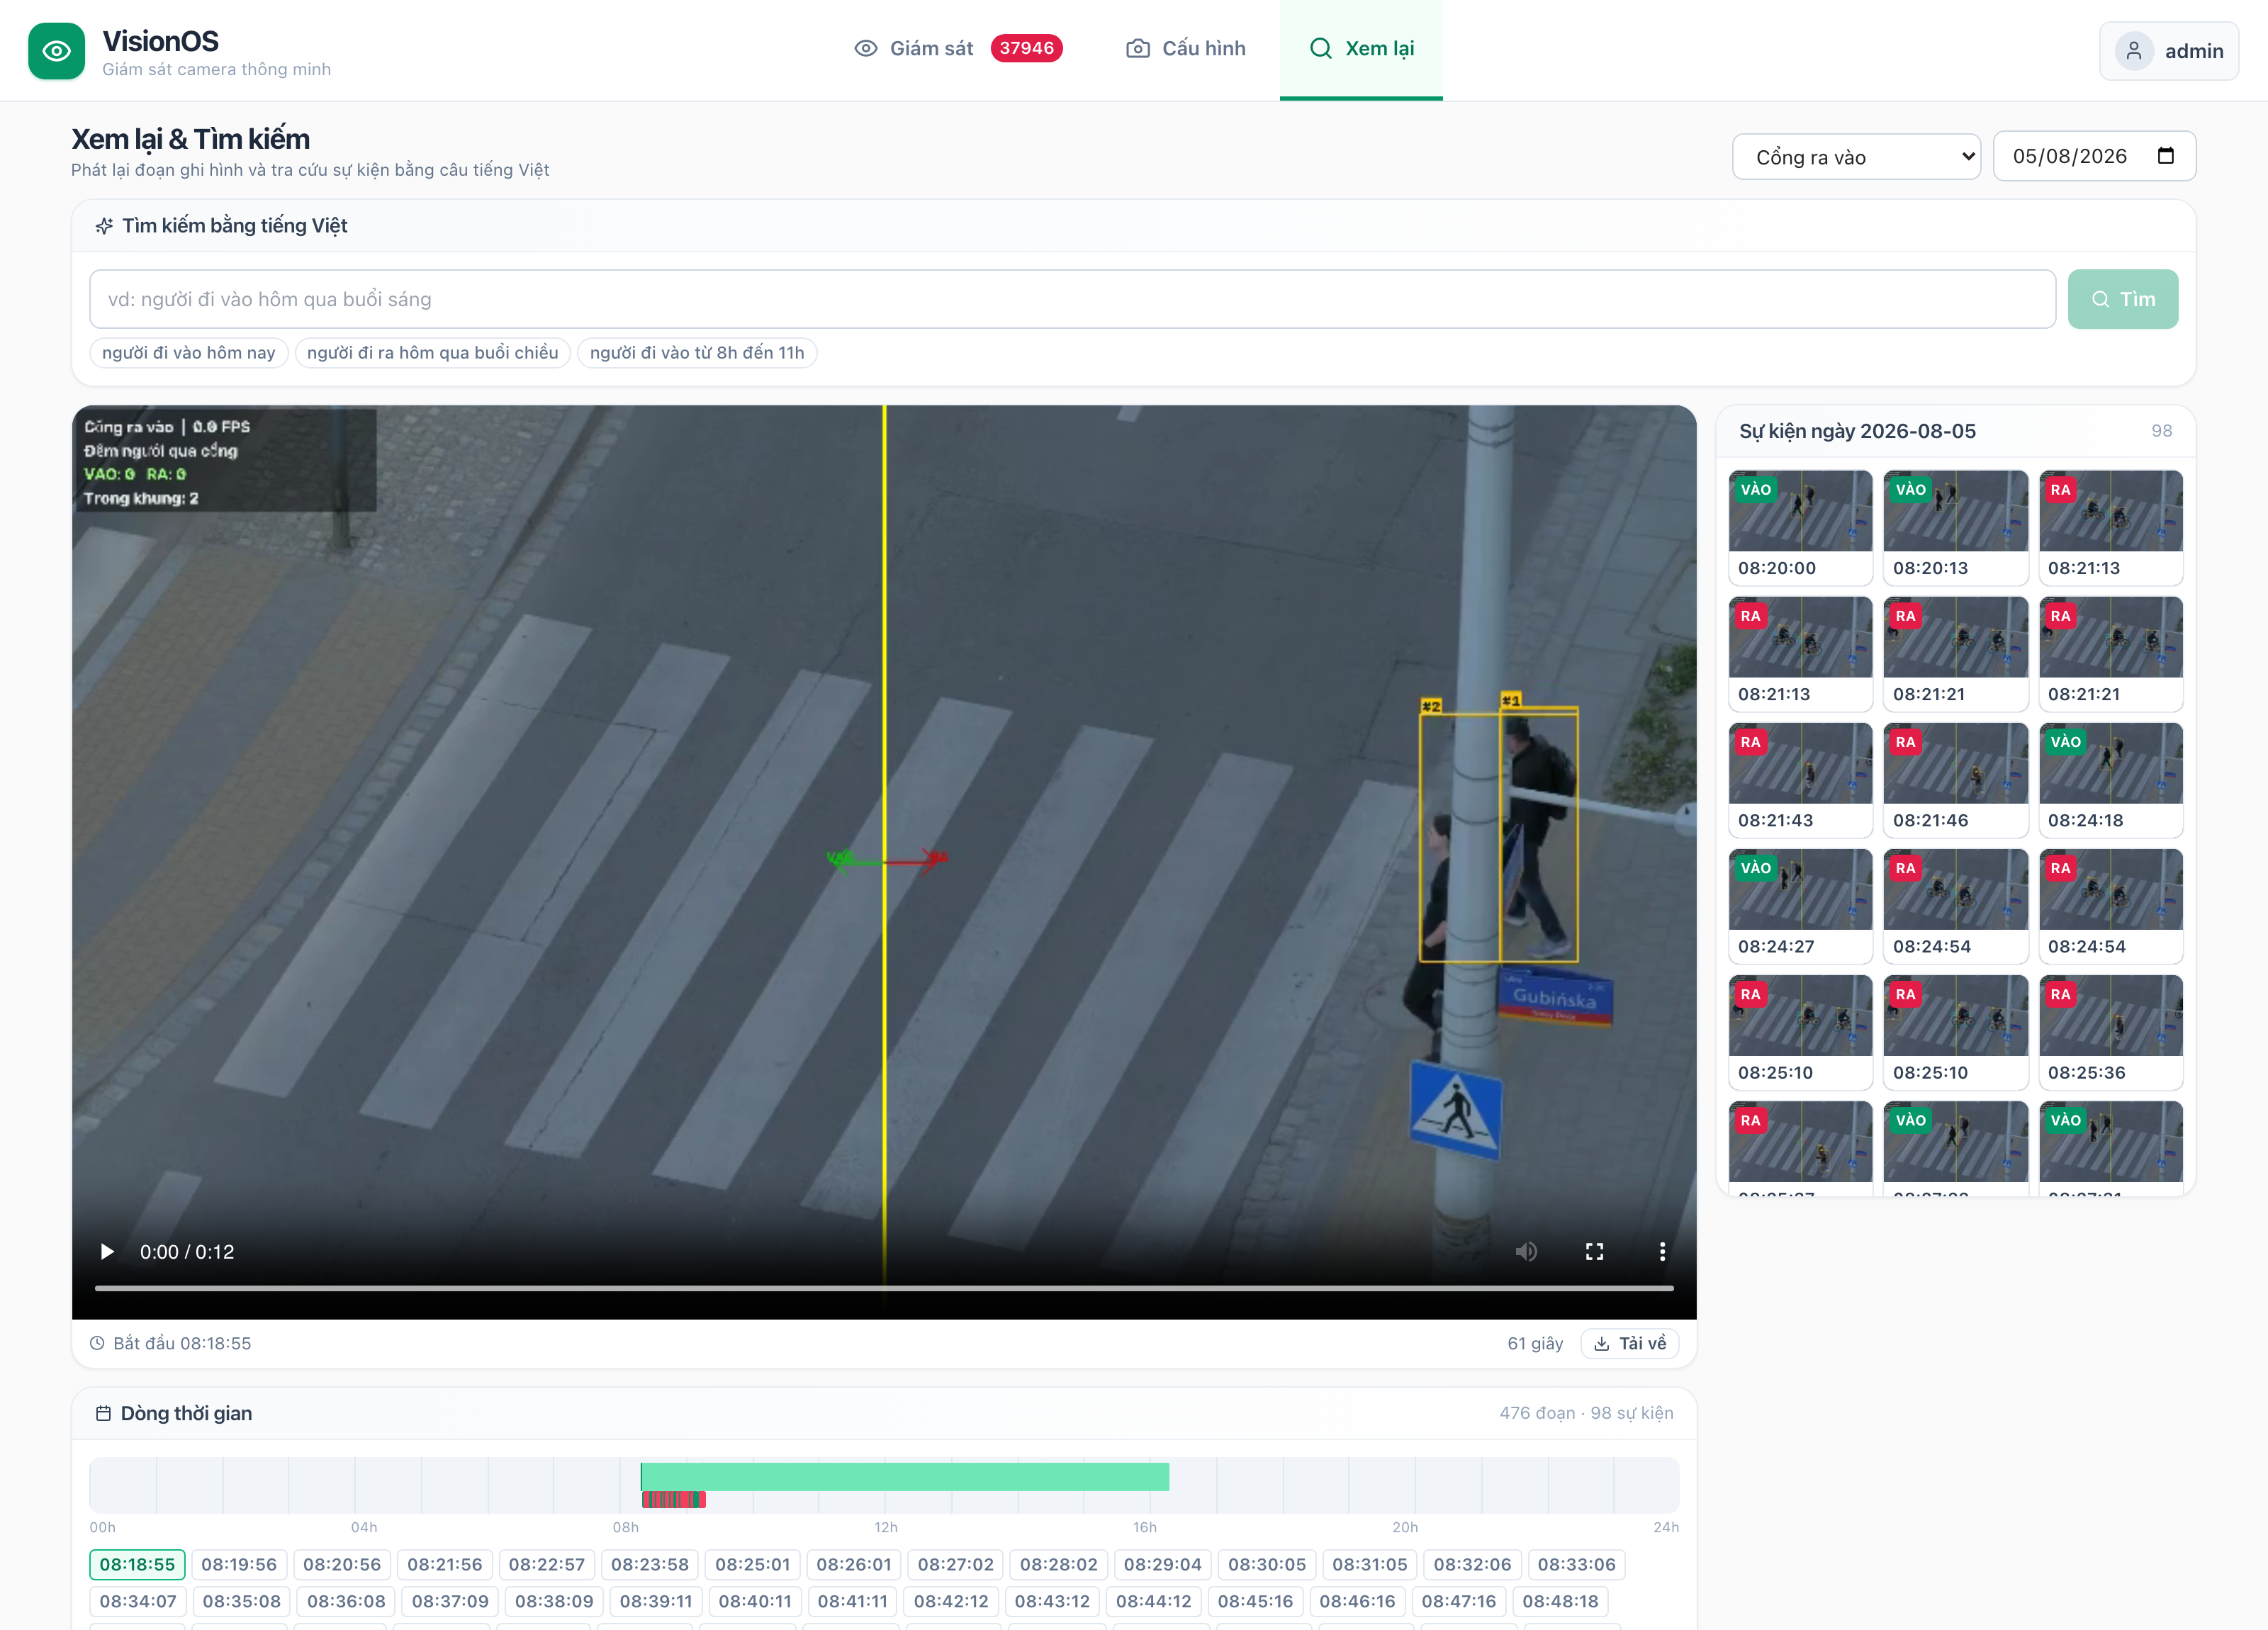
\includegraphics[width=\textwidth]{figures/ui_playback.png}
\caption{Trang xem lại. Thanh thời gian gộp cả vùng đã ghi hình lẫn vị trí sự
kiện; bấm vào một vạch sự kiện sẽ tua video tới đúng giây đó.}
\label{fig:ui-playback}
\end{figure}

\subsubsection*{Tách việc ghi nhận khỏi việc đếm}
\label{sub:ghi-va-dem}

Bản đầu chỉ ghi sự kiện cho đúng những lớp đối tượng và đúng chiều mà pipeline
được cấu hình để đếm. Hệ quả là muốn về sau tra cứu được xe đạp thì phải đoán
trước từ lúc dựng pipeline, còn không thì dữ liệu vĩnh viễn không tồn tại. Điều
này mâu thuẫn với cách trang xem lại tự giới thiệu: người dùng chọn camera và
chọn ngày, không ai nghĩ kết quả lại phụ thuộc vào một cấu hình đặt từ tuần
trước.

Câu hỏi tự nhiên là vì sao không quét thẳng trên video lúc tìm kiếm. Phép đo trả
lời dứt điểm: trên đoạn ghi hình 854$\times$1518, tốc độ quét đạt 12,3 khung mỗi
giây, tức quét một phút video mất 49 giây. Riêng dữ liệu của một ngày --- 862
phút --- cần gần 12 giờ. Tìm kiếm phải đọc bảng đã tính sẵn, không có cách nào
khác.

Nhưng phép đo thứ hai mới là chỗ đáng nói:

\begin{table}[H]
\centering
\begin{tabular}{lrr}
\toprule
\textbf{Số lớp yêu cầu} & \textbf{Thời gian} & \textbf{Tốc độ} \\
\midrule
1 lớp (chỉ Người) & 3,25 s & 12,3 khung/giây \\
6 lớp (người, xe đạp, ô tô, xe máy, xe buýt, xe tải) & 3,17 s & 12,6 khung/giây \\
\bottomrule
\end{tabular}
\caption{Chi phí suy luận không phụ thuộc số lớp yêu cầu}
\label{tab:chi-phi-lop}
\end{table}

Chênh lệch 2,5\%, nằm trong sai số. Lý do là YOLO tính điểm cho toàn bộ tám mươi
lớp trong một lượt truyền xuôi duy nhất; tham số \code{classes} chỉ lọc bỏ kết
quả \emph{sau} khi đã tính xong. Nói cách khác, mỗi lần camera thấy một chiếc xe
đạp thì mô hình đã nhận ra nó rồi, và hệ thống chủ động vứt đi. Đây không phải
giới hạn tài nguyên mà là một quyết định thiết kế sai.

Cách sửa là tách hai khái niệm vốn bị gộp làm một: \emph{ghi nhận cái gì} và
\emph{đếm cái gì}. Bộ đếm nhận thêm tham số \code{count\_labels}; mọi lượt cắt
vạch đều được ghi kèm nhãn thật của nó, nhưng chỉ những lượt khớp cả lớp lẫn
chiều người dùng chọn mới cộng vào con số hiển thị.

Trong lúc kiểm chứng lộ ra rằng bộ lọc chiều cũng mắc đúng lỗi ấy: pipeline đặt
``chỉ đếm vào'' thì mọi lượt đi ra bị loại thẳng khỏi danh sách sự kiện, nên tìm
``người đi ra hôm nay'' trên camera đó không ra gì dù hệ thống đã nhìn thấy đủ.
Sửa cùng nguyên tắc.

Đo trên video lối đi bộ với đúng cấu hình pipeline đang chạy (chỉ đếm Người,
chỉ chiều Vào):

\begin{table}[H]
\centering
\begin{tabular}{lrr}
\toprule
& \textbf{Trước} & \textbf{Sau} \\
\midrule
Số đếm hiển thị & vào 2, ra 0 & vào 2, ra 0 \\
Sự kiện tra cứu được & 2 & 8 \\
\quad trong đó xe đạp & 0 & 2 \\
\quad trong đó lượt đi ra & 0 & 6 \\
\bottomrule
\end{tabular}
\caption{Số đếm giữ nguyên, dữ liệu tra cứu tăng gấp bốn}
\label{tab:ghi-va-dem}
\end{table}

Một chi tiết đáng chú ý ở khung 497 và 532: xe đạp và người cùng cắt vạch trong
một khung hình, vì đó là một người đang đạp xe. Ghi cả hai thì về sau tra cứu
được theo cả hai cách, còn chỉ đếm Người nên một thực thể không bị đếm thành hai.
Đây chính là lý do phải tách hai khái niệm thay vì mở rộng danh sách lớp đếm.

\subsubsection*{Bốn lỗi trong bộ phân tích câu lệnh tiếng Việt}
\label{sub:loi-tim-kiem}

Kiểm thử tìm kiếm bằng ba mươi mấy câu lệnh, mỗi câu vừa xét xem hệ thống hiểu
gì vừa đối chiếu từng kết quả trả về với bộ lọc, đã lộ ra bốn lỗi cùng một họ.

Gốc chung của cả bốn là việc dò từ khoá bằng phép kiểm chuỗi con trên văn bản đã
bỏ dấu. Tiếng Việt bỏ dấu thì nhiều từ khác hẳn nhau lại trùng nhau: ``tối'',
``tôi'' và ``tới'' đều thành \code{toi}; còn chính chữ \code{camera} thì chứa sẵn
\code{ra}.

\begin{table}[H]
\centering
\begin{tabular}{lll}
\toprule
\textbf{Câu người dùng gõ} & \textbf{Hệ thống hiểu} & \textbf{Đúng ra phải là} \\
\midrule
\emph{người đi ra tối qua}  & hôm nay buổi tối & hôm qua buổi tối \\
\emph{camera của tôi}       & chiều ra, 18h--24h & không có tiêu chí nào \\
\emph{người đi vào tới 15h} & hôm nay buổi tối & không nhận ra \\
\emph{người đi vào lúc 12h} & bỏ qua phần giờ & 12h--13h \\
\bottomrule
\end{tabular}
\caption{Bốn lỗi phát hiện khi kiểm thử tìm kiếm tiếng Việt}
\label{tab:loi-tim-kiem}
\end{table}

Điểm nguy hiểm không nằm ở chỗ hiểu sai, mà ở chỗ hiểu sai một cách \emph{tự
tin}: dòng ``đã hiểu'' trên giao diện vẫn liệt kê đầy đủ tiêu chí, nên người dùng
không có cách nào biết kết quả đã bị cắt theo một khung giờ họ không hề yêu cầu.
Câu ``camera của tôi'' đáng lẽ trả về mọi sự kiện thì lại chỉ trả về khoảng
18h--24h của hôm nay.

Sửa bằng cách thay toàn bộ phép kiểm chuỗi con bằng so khớp theo ranh giới từ,
bổ sung hư từ vào danh sách từ dừng, nhận thêm dạng ``buổi + qua/nay'' để phân
biệt tối hôm qua với tối hôm nay, và siết điều kiện dò tên camera --- trước đây
chỉ cần một chữ ba ký tự trùng ở bất kỳ đâu trong tên hay vị trí, nên chữ
``của'' khớp ngay với camera ``Cửa tàu điện ngầm''.

Riêng những dạng chưa xử lý được như ``từ 8h'', ``trước 14h'' thì để hệ thống báo
thẳng là không nhận ra tiêu chí, thay vì đoán bừa thành một khung giờ. Với một
công cụ tra cứu, im lặng trả về kết quả sai nguy hiểm hơn nhiều so với việc thừa
nhận không hiểu câu hỏi.

Sau khi sửa, ba bộ kiểm chạy sạch: 17 câu về thời gian, 11 câu về nhận nhầm
chiều và camera, 19 câu đầu--cuối có đối chiếu từng kết quả với bộ lọc.

\section{Kết quả thực nghiệm}
\label{sec:thucnghiem}

Môi trường đo: Apple M4, 24~GB bộ nhớ, macOS~26.4, Python~3.12, PyTorch~2.13
chạy trên MPS, trọng số \code{yolov8n.pt}, kích thước ảnh vào 960 điểm ảnh.

\subsection{Ảnh hưởng của ngưỡng ghép vết ByteTrack}

Thí nghiệm chạy trên \code{walkback.mp4} (2160$\times$3840, 24~fps, 480 khung
hình, hai người trong cảnh), giữ nguyên mọi tham số khác và chỉ đổi
\code{minimum\_matching\_threshold}.

\begin{table}[H]
\centering
\caption{Ngưỡng ghép vết quyết định độ bền của track. Giá trị 0{,}3 làm vết vỡ
vụn thành 65 mảnh dù cảnh chỉ có hai người.}
\label{tab:bytetrack}
\small
\begin{tabular}{@{}rrrrrr@{}}
\toprule
\textbf{Ngưỡng} & \textbf{IoU tối thiểu} & \textbf{Số mã ID} &
\textbf{Độ dài trung vị} & \textbf{Vào} & \textbf{Ra} \\
\midrule
0{,}3 & 0{,}7 & 65 & 2 khung   & 2 & 2 \\
0{,}5 & 0{,}5 & 2  & 480 khung & 2 & 2 \\
0{,}7 & 0{,}3 & 2  & 480 khung & 2 & 2 \\
0{,}8 & 0{,}2 & 2  & 480 khung & 2 & 2 \\
0{,}9 & 0{,}1 & 2  & 480 khung & 2 & 2 \\
\bottomrule
\end{tabular}
\end{table}

Ở ngưỡng 0{,}3, hai người sinh ra 65 mã định danh với độ dài trung vị chỉ hai
khung hình. Từ 0{,}5 trở lên, mỗi người giữ đúng một mã suốt cả đoạn video.

Số đếm vẫn đúng bằng 2 ở mọi ngưỡng, kể cả 0{,}3. Kết quả này cho thấy cơ chế nối
lại vết theo không gian mô tả ở Mục~\ref{sec:dem} bù được phần lớn thiệt hại do
vết đứt gãy. Hệ thống vẫn đặt mặc định 0{,}9 vì vết liền mạch giúp ảnh chụp sự
kiện và mã định danh hiển thị trên màn hình có ý nghĩa với người xem.

\subsection{Điểm neo: bàn chân so với tâm hộp}

Cùng đoạn video hai người, so sánh hai lựa chọn điểm neo ở các vị trí vạch khác
nhau. Cột \emph{tâm hộp} tắt luôn vùng đệm và độ trễ xác nhận, tái hiện đúng cách
làm của \code{LineZone} nguyên bản.

\begin{table}[H]
\centering
\caption{Điểm neo bàn chân loại bỏ hiện tượng đếm dư. Với vạch dọc giữa khung,
tâm hộp báo 5 lượt mỗi chiều trong khi cảnh chỉ có hai người.}
\label{tab:anchor}
\small
\begin{tabular}{@{}lcccc@{}}
\toprule
\multirow{2}{*}{\textbf{Vị trí vạch}} &
\multicolumn{2}{c}{\textbf{Điểm neo bàn chân}} &
\multicolumn{2}{c}{\textbf{Tâm hộp}} \\
\cmidrule(lr){2-3}\cmidrule(lr){4-5}
 & \textbf{Vào} & \textbf{Ra} & \textbf{Vào} & \textbf{Ra} \\
\midrule
Ngang 40\% & 0 & 0 & 0 & 0 \\
Ngang 50\% & 0 & 0 & 2 & 2 \\
Ngang 60\% & \textbf{2} & \textbf{2} & 0 & 0 \\
Ngang 70\% & 0 & 0 & 0 & 0 \\
Dọc 30\%   & 0 & 0 & 0 & 0 \\
Dọc 50\%   & 0 & 0 & \textbf{5} & \textbf{5} \\
Dọc 70\%   & 0 & 0 & 1 & 1 \\
\bottomrule
\end{tabular}
\end{table}

Hàng \emph{dọc 50\%} là trường hợp đáng chú ý nhất. Hai người trong cảnh đi dọc
theo phương của vạch chứ không cắt qua nó, nên đáp án đúng là không đếm lượt nào.
Điểm neo bàn chân cho đúng 0. Tâm hộp báo 5 lượt vào và 5 lượt ra, toàn bộ sinh ra
từ dao động của tâm hộp khi kích thước hộp thay đổi theo bước chân.

Ở vạch ngang 60\%, điểm neo bàn chân cho kết quả 2 vào và 2 ra, khớp với nội dung
đoạn video: hai người đi khỏi camera rồi quay lại.

Vị trí vạch ảnh hưởng mạnh không kém lựa chọn điểm neo. Cùng điểm neo bàn chân,
vạch ở 50\% và 70\% chiều cao đều cho 0, chỉ vạch ở 60\% mới bắt được đúng chỗ
bàn chân đi qua. Đây là lý do giao diện cho phép kéo vạch trực tiếp trên ảnh thay
vì cố định ở giữa khung hình.

\subsection{Luồng Thông minh: chi phí và khả năng lọc}

Thí nghiệm chạy trên một khung hình có hai người, cắt hộp rồi hỏi bộ lọc thông minh bốn truy vấn
khác nhau.

\begin{table}[H]
\centering
\caption{Khả năng lọc thuộc tính trên khung hình hai người. Lần
gọi đầu tiên chậm do khởi động, các lần sau ổn định ở khoảng 1,2 giây cho hai khung cắt.}
\label{tab:la3b}
\small
\begin{tabular}{@{}lcc@{}}
\toprule
\textbf{Truy vấn} & \textbf{Số khung cắt giữ lại} & \textbf{Thời gian} \\
\midrule
\code{person}                  & 2/2 & 5,4 s (có khởi động) \\
\code{person with backpack}    & 2/2 & 1,2 s \\
\code{person in red shirt}     & 1/2 & 1,2 s \\
\code{person holding umbrella} & 1/2 & 1,2 s \\
\bottomrule
\end{tabular}
\end{table}

Mô hình phân biệt được thuộc tính: truy vấn \code{person} giữ cả hai người, còn
\code{red shirt} và \code{umbrella} chỉ giữ một. Riêng \code{backpack} giữ cả hai, tức
là có nhận nhầm --- xem phần hạn chế ở Mục~\ref{sec:hanche}.

Đo trên luồng camera đang chạy thật với câu lệnh \emph{"người mặc áo trắng"}: hệ thống
gọi LA-3B 9 lần, kết quả 4 khớp và 5 bị loại, tốc độ xử lý giữ ở \textbf{18 khung hình
mỗi giây}. So với 45 khung hình mỗi giây của luồng Tiêu chuẩn trên cùng nguồn video, chi
phí giảm khoảng 60\% nhưng vẫn dư so với nhịp 15 khung hình mỗi giây mà hệ thống đặt làm
mục tiêu. Con số này chỉ đạt được nhờ ba cơ chế mô tả ở Mục~\ref{sec:thongminh}; gọi
LA-3B trực tiếp trong vòng lặp sẽ kéo tốc độ xuống dưới 1 khung hình mỗi giây.

Mô hình nạp trong 11,9 giây và chiếm 8,2~GB bộ nhớ GPU.

\subsection{Cách diễn đạt truy vấn quyết định chất lượng lọc}
\label{sec:cachdien}

Thí nghiệm này xuất phát từ một lỗi người dùng báo: gõ \emph{"người đeo túi"} nhưng hệ
thống giữ lại cả người có túi lẫn người không.

Chọn một khung hình ở sảnh nhà ga có 37 người, cắt hộp rồi hỏi cùng một nội dung nhưng
diễn đạt theo hai cách khác nhau.

\begin{table}[H]
\centering
\caption{Câu truy vấn bắt đầu bằng chủ ngữ chỉ người gần như không lọc được gì. Đưa
thẳng vật thể thì mô hình mới thực sự đi tìm vật thể đó.}
\label{tab:truyvan}
\small
\begin{tabular}{@{}llcc@{}}
\toprule
\textbf{Người dùng gõ} & \textbf{Truy vấn đưa vào} & \textbf{Giữ lại} & \textbf{Tỉ lệ} \\
\midrule
--- & \code{person} (nền) & 36/37 & 97\% \\
\midrule
người đeo ba lô & \code{person with backpack} & 32/37 & 86\% \\
người đeo ba lô & \code{backpack} & \textbf{9/37} & \textbf{24\%} \\
\addlinespace
người xách túi & \code{handbag man} & 34/37 & 92\% \\
người xách túi & \code{handbag} & \textbf{14/37} & \textbf{38\%} \\
\addlinespace
người đeo túi & \code{the man with the bag} & 29/37 & 78\% \\
người đeo túi & \code{bag} & \textbf{16/37} & \textbf{43\%} \\
\addlinespace
người cầm ô & \code{person holding umbrella} & 7/37 & 19\% \\
người cầm ô & \code{umbrella} & \textbf{0/37} & \textbf{0\%} \\
\bottomrule
\end{tabular}
\end{table}

Khi câu bắt đầu bằng \code{person}, mô hình bám vào chính chữ đó và gần như bỏ qua vế
mô tả phía sau: tỉ lệ giữ lại 78--92\%, chỉ nhỉnh hơn chút so với mức 97\% của truy vấn
\code{person} thuần. Bỏ chủ ngữ đi, chỉ để lại vật thể, tỉ lệ tụt xuống 24--43\%.

Hàng cuối là phép thử đối chứng: sảnh nhà ga trong nhà, không ai cầm ô. Truy vấn
\code{umbrella} trả về đúng 0, còn \code{person holding umbrella} vẫn nhận nhầm 7 người.

Để kiểm tra xem 24\% kia có thật sự đúng hay chỉ là lọc bừa, tôi ghép ảnh các khung cắt
được giữ lại và các khung bị loại rồi đối chiếu bằng mắt. Cả 9 khung được giữ với truy
vấn \code{backpack} đều là người thật sự mang ba lô hoặc túi cỡ lớn; phần lớn khung bị
loại là người tay không hoặc chỉ xách túi nhỏ. Đây là hành vi đúng của từ
\emph{backpack}.

Kết quả này dẫn tới thay đổi trong tầng dịch: từ điển Việt--Anh giờ ánh xạ
\emph{"người đeo ba lô"} thành \code{backpack} chứ không phải \code{person with
backpack}, và bản dịch tự động cũng bị cắt bỏ phần chủ ngữ đứng đầu trước khi dùng.

\subsection{Hiệu chỉnh vùng đệm của bộ đếm}
\label{sec:hieuchinh-vungdem}

Sáu pipeline đếm qua vạch trên năm video mẫu được dùng làm bộ kiểm thử. Do suy luận
YOLO chiếm gần hết thời gian chạy, kết quả phát hiện của mỗi video được lưu đệm ra
tệp \code{.pkl}; các lần quét tham số sau đó chỉ chạy lại phần đếm, nhờ vậy một lượt
quét đầy đủ mất vài giây thay vì vài chục phút.

Chuẩn đối chiếu không lấy từ số đếm mà từ bốn lượt đã kiểm tra bằng mắt trên ảnh cắt
sát từng người: ba lượt đi qua thật (một người vào cửa hàng tiện lợi, hai người đi
qua cửa sảnh ga ra ngoài) và một người đứng xếp hàng cạnh vạch ở ga tàu điện ngầm
--- trường hợp bắt buộc không được đếm.

\begin{table}[H]
\centering
\caption{Quét hệ số vùng đệm và độ trễ xác nhận. Chỉ cấu hình 0{,}03 với ba khung
xác nhận không mắc sai sót nào; các mức rộng hơn bỏ sót lượt đi qua thật.}
\label{tab:vungdem}
\small
\begin{tabularx}{\textwidth}{@{}rrX@{}}
\toprule
\textbf{Hệ số} & \textbf{Độ trễ} & \textbf{Sai sót so với chuẩn đối chiếu} \\
\midrule
0{,}12 & 3--8 & Bỏ sót cả ba lượt đi qua thật \\
0{,}08 & 3--5 & Bỏ sót hai lượt \\
0{,}05 & 3     & Bỏ sót một lượt \\
\textbf{0{,}03} & \textbf{3} & \textbf{Không có} \\
0{,}02 & 3     & Không có, nhưng chặt hơn mà không thêm lợi ích \\
\bottomrule
\end{tabularx}
\end{table}

\begin{table}[H]
\centering
\caption{Số đếm trước và sau khi đổi hệ số vùng đệm từ 0{,}12 xuống 0{,}03. Ba lượt
đi qua thật bị bỏ sót trước đây nay được đếm đúng.}
\label{tab:truocsau}
\small
\begin{tabularx}{\textwidth}{@{}Xccc@{}}
\toprule
\textbf{Pipeline} & \textbf{Trước} & \textbf{Sau} & \textbf{Ghi chú} \\
\midrule
Đếm người qua cửa hàng          & 0/0 & \textbf{1/0}  & Bắt được lượt vào cửa \\
Đếm người qua cửa sảnh ga       & 1/3 & \textbf{1/5}  & Bắt được hai lượt ra \\
Đếm qua vạch --- Cửa tàu điện   & 5/9 & 6/10 & Mã vết bị trôi \\
Đếm qua vạch --- người đeo túi  & 8/5 & 9/6  & Mã vết bị trôi \\
Đếm người mặc áo trắng          & 2/4 & 2/4  & Không đổi \\
Đếm người qua cổng              & 2/4 & 2/4  & Không đổi \\
\bottomrule
\end{tabularx}
\end{table}

Trường hợp quyết định là camera cửa hàng tiện lợi. Người trong cảnh đứng sát camera
nên hộp giới hạn cao 1178 điểm ảnh, trong khi cả quãng bước từ vỉa hè vào trong cửa
chỉ đưa bàn chân dịch 288 điểm ảnh theo phương vuông góc với vạch, và chỉ vượt qua
vạch được 60 điểm ảnh trước khi người đó khuất vào bên trong. Với hệ số 0{,}12, dải
đệm rộng 141 điểm ảnh --- lượt đi vào thật bị bỏ. Với hệ số 0{,}03, dải đệm rộng 35
điểm ảnh và lượt này được đếm đúng.

Bài học rút ra là bằng chứng \emph{đã đi qua thật} không nên đến từ việc đối tượng đi
\emph{xa} vạch, vì quãng đường theo phương vuông góc phụ thuộc vào góc đặt camera chứ
không phản ánh hành vi. Bằng chứng đến từ trung bình trượt mười khung hình cộng với
yêu cầu giữ nguyên phía mới trong ba khung liên tiếp. Dải đệm chỉ cần đủ rộng để chặn
nhiễu của hộp giới hạn.

\begin{figure}[H]
\centering
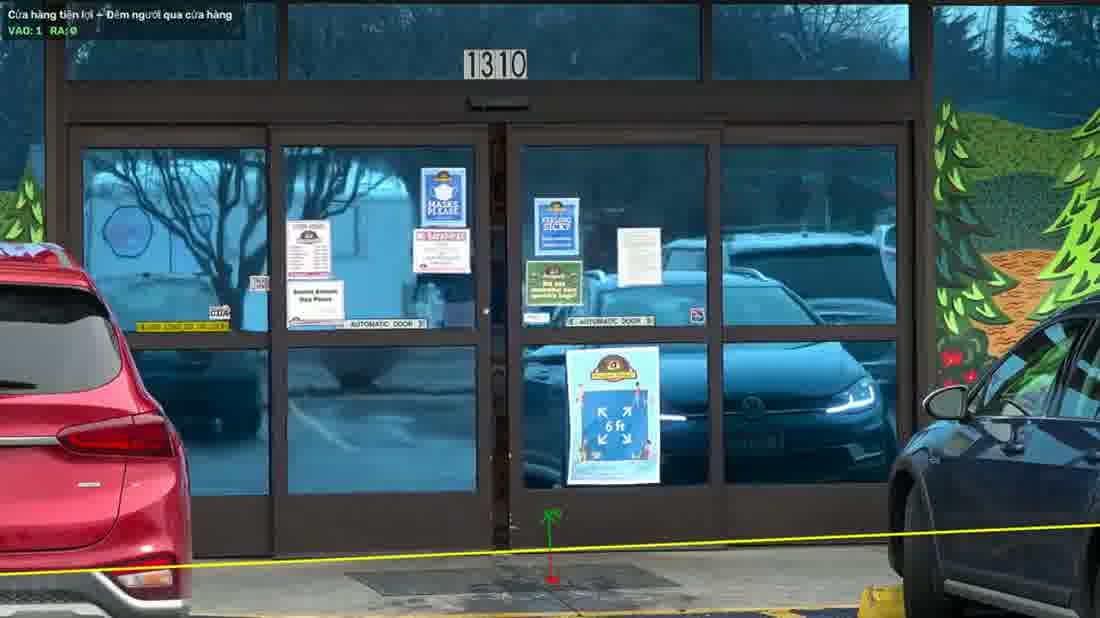
\includegraphics[width=0.86\textwidth]{figures/dem_cua_hang.jpg}
\caption{Camera cửa hàng tiện lợi sau khi hiệu chỉnh. Vạch ngang nằm ở ngưỡng cửa,
mũi tên chỉ chiều Vào hướng vào trong cửa hàng, bảng đếm ghi nhận đúng một lượt vào.}
\label{fig:demcuahang}
\end{figure}

\begin{figure}[H]
\centering
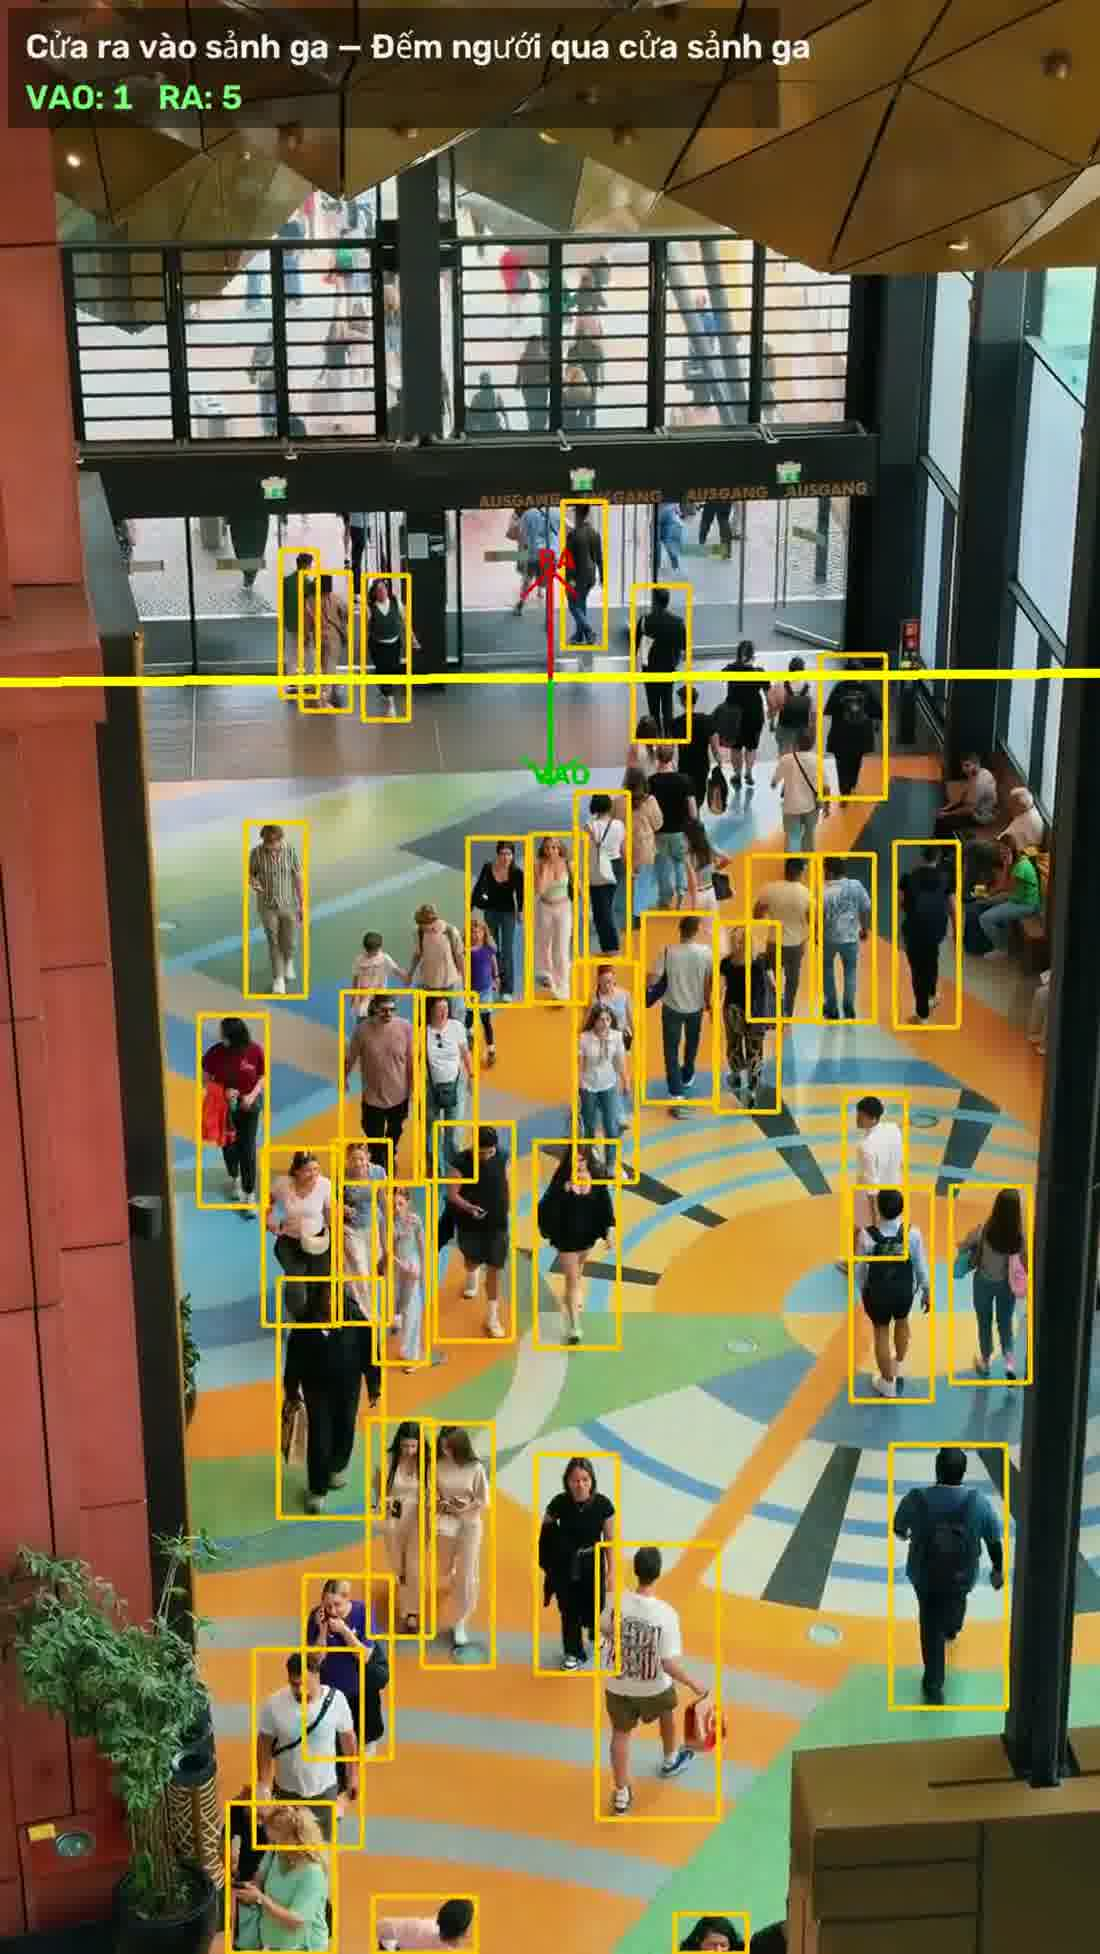
\includegraphics[height=0.52\textheight]{figures/dem_sanh_ga.jpg}
\caption{Camera cửa ra vào sảnh ga, khung hình cuối đoạn. Vạch ngang đặt ngay dưới
dãy cửa thoát, mũi tên Ra hướng về phía cửa. Đây là cảnh đông nhất trong bộ kiểm
thử, trung bình 39 người mỗi khung hình.}
\label{fig:demsanhga}
\end{figure}

Hai pipeline trên video ga tàu điện ngầm tăng thêm một lượt mỗi chiều. Nguyên nhân đã
truy được: một mã vết tồn tại 694 khung hình nhưng bị ByteTrack gán lần lượt cho nhiều
người khác nhau trong đám đông, sinh ra ba lượt cắt vạch trong khi không ai đi qua ba
lần. Đây là hạn chế của khâu bám vết ở cảnh dày đặc, không phải của bộ đếm. Kéo dài
thời gian chống đếm lặp lên 250 khung hình dập được hiện tượng này, nhưng cách đó bị
loại vì thời gian chống đếm lặp tính theo khung hình: 250 khung là 4{,}2 giây ở video
60~fps nhưng 10 giây ở video 25~fps, khiến hành vi thay đổi theo tốc độ nguồn --- và
quan trọng hơn, nó chỉ che triệu chứng của một khiếm khuyết nằm ở nơi khác.

\subsection{Độ chính xác đo bằng nhãn chuẩn MOT17}
\label{sec:mot17}

Các phép kiểm ở trên đều đối chiếu bằng mắt trên vài vết, nên chỉ trả lời được ``có sai
ở chỗ này không'' chứ không cho ra con số. Mục này dùng bộ dữ liệu bám vết công khai
MOT17, trong đó \emph{mỗi khung hình đã có sẵn hộp giới hạn, mã vết và độ nhìn thấy do
người gán}, nên số lượt qua bất kỳ vạch nào cũng tính ra chính xác được.

Ba chuỗi camera tĩnh của MOT17 dùng được. Bốn chuỗi còn lại quay bằng máy di động nên
vạch đếm trôi theo khung hình, bài toán không định nghĩa được.

\subsubsection*{Cách so sánh}

Danh sách lượt qua vạch đúng được sinh từ nhãn chuẩn bằng \emph{đúng công thức khoảng
cách có dấu và vùng đệm mà bộ đếm dùng}. Sau đó mỗi lượt của hệ thống được ghép với
lượt gần nhất trong nhãn chuẩn: cùng chiều, lệch dưới 45 khung hình và 200 điểm ảnh.
Ghép được là đếm đúng, không ghép được là đếm thừa, còn dư trong nhãn chuẩn là bỏ sót.

Dùng chung công thức là bắt buộc. Lần chạy đầu tiên tôi tự viết lại phép tính chiều
theo quy ước riêng; với vạch dọc thì dấu bị ngược so với bộ đếm nên mọi lượt đều lệch
chiều và không ghép được cặp nào, cho ra ``độ chính xác 27\%'' trong khi tổng số lượt
hai bên chỉ chênh nhau đúng một.

\begin{table}[H]
\centering
\caption{Độ chính xác đếm ở cấu hình vạch tốt nhất của từng chuỗi. Ghép cặp chặt: cùng
chiều, lệch dưới 1{,}5 giây và 200 điểm ảnh.}
\label{tab:mot17}
\small
\begin{tabularx}{\textwidth}{@{}Xrrrrrrrr@{}}
\toprule
\textbf{Chuỗi} & \textbf{Chuẩn} & \textbf{Hệ thống} & \textbf{Khớp} &
\textbf{Thừa} & \textbf{Sót} & \textbf{Độ phủ} & \textbf{Độ chuẩn} & \textbf{F1} \\
\midrule
MOT17-02 & 15 & 12 & 11 & 1 & 4 & 73\% & 92\% & 0{,}81 \\
MOT17-04 & 15 & 15 & \textbf{15} & \textbf{0} & \textbf{0} & \textbf{100\%} & \textbf{100\%} & \textbf{1{,}00} \\
MOT17-09 & 13 & 12 & 12 & 0 & 1 & 92\% & 100\% & 0{,}96 \\
\midrule
\textbf{Cộng} & \textbf{43} & \textbf{39} & \textbf{38} & \textbf{1} & \textbf{5} &
\textbf{88\%} & \textbf{97\%} & \textbf{0{,}92} \\
\bottomrule
\end{tabularx}
\end{table}

Trên 43 lượt qua vạch có nhãn chuẩn, hệ thống đếm đúng 38 lượt, đếm thừa 1 và bỏ sót 5.

\subsubsection*{Độ chính xác đi theo độ nhìn thấy, không theo mật độ}

\begin{table}[H]
\centering
\caption{Đặc điểm ba cảnh. Chuỗi đông người nhất lại chính xác nhất; thứ tự F1 khớp
hoàn toàn với thứ tự độ nhìn thấy.}
\label{tab:mot17-canh}
\small
\begin{tabularx}{\textwidth}{@{}Xrrrr@{}}
\toprule
\textbf{Chuỗi} & \textbf{Người/khung} & \textbf{Độ nhìn thấy} &
\textbf{Cao trung vị} & \textbf{F1} \\
\midrule
MOT17-02 --- Quảng trường  & 11{,}2 & 40\% & 171 px & 0{,}81 \\
MOT17-09 --- Vỉa hè        &  9{,}5 & 59\% & 285 px & 0{,}96 \\
MOT17-04 --- Phố đêm       & \textbf{25{,}7} & \textbf{62\%} & 175 px & \textbf{1{,}00} \\
\bottomrule
\end{tabularx}
\end{table}

MOT17-04 đông gấp 2{,}7 lần MOT17-09 nhưng chính xác hơn. Đông người không phải vấn đề;
\textbf{che khuất} mới là vấn đề. Camera của MOT17-04 đặt trên cao nên người ít che
nhau, còn MOT17-02 đặt ngang tầm mắt nhìn dọc một con phố dài, hàng chục người ở xa
nhỏ như hạt gạo và che lấp nhau liên tục.

\subsubsection*{Lỗi nằm ở khâu phát hiện, không ở khâu đếm}

Đo riêng độ phủ của khâu phát hiện --- tỉ lệ hộp trong nhãn chuẩn mà YOLO tìm được với
$\text{IoU} \geq 0{,}5$:

\begin{table}[H]
\centering
\caption{Độ phủ phát hiện thấp hơn hẳn độ chính xác đếm. Tính riêng dải quanh vạch thì
cao hơn nhiều so với toàn khung hình.}
\label{tab:mot17-phathien}
\small
\begin{tabularx}{\textwidth}{@{}Xrrrr@{}}
\toprule
\multirow{2}{*}{\textbf{Chuỗi}} & \multicolumn{2}{c}{\textbf{Toàn khung hình}} &
\multicolumn{2}{c}{\textbf{Dải quanh vạch $\pm$120 px}} \\
\cmidrule(lr){2-3}\cmidrule(lr){4-5}
 & \textbf{Số hộp} & \textbf{Độ phủ} & \textbf{Số hộp} & \textbf{Độ phủ} \\
\midrule
MOT17-02 & 18\,581 & 37\% & 2\,318 & 44\% \\
MOT17-04 & 47\,557 & 54\% & 3\,629 & \textbf{76\%} \\
MOT17-09 &  5\,325 & 80\% &   287 & \textbf{84\%} \\
\bottomrule
\end{tabularx}
\end{table}

YOLOv8n bỏ sót hơn một nửa số người có trong nhãn chuẩn, nhưng đếm vẫn đạt 0{,}81 đến
1{,}00. Không có mâu thuẫn ở đây: đếm qua vạch chỉ cần thấy một người \emph{đúng lúc họ
bước qua vạch}, không cần thấy họ suốt video. Một người bị bỏ sót ở chín phần mười số
khung vẫn được đếm đúng nếu hiện ra ở vài khung quanh vạch.

Hệ quả cho việc đánh giá: \textbf{độ phủ phát hiện toàn khung hình là chỉ số sai} để
đo chất lượng một hệ thống đếm. Chỉ số đúng là độ phủ \emph{tại vạch}, và cột bên phải
Bảng~\ref{tab:mot17-phathien} cho thấy nó cao hơn đáng kể.

Truy tiếp vào từng lượt bỏ sót thì nguyên nhân lộ rõ:

\begin{table}[H]
\centering
\caption{Độ nhìn thấy tại thời điểm qua vạch. Lượt bỏ sót luôn có độ nhìn thấy thấp
hơn hẳn lượt đếm đúng.}
\label{tab:mot17-sot}
\small
\begin{tabularx}{\textwidth}{@{}Xcc@{}}
\toprule
\textbf{Chuỗi} & \textbf{Khi đếm đúng} & \textbf{Khi bỏ sót} \\
\midrule
MOT17-02 & 71\% & 58\% \\
MOT17-04 & 82\% & --- (không sót lượt nào) \\
MOT17-09 & 60\% & \textbf{0\%} \\
\bottomrule
\end{tabularx}
\end{table}

Lượt bỏ sót duy nhất của MOT17-09 có độ nhìn thấy \textbf{0\%}: người đó bị che hoàn
toàn đúng khoảnh khắc bước qua vạch. Không mô hình phát hiện nào cứu được trường hợp
này --- đây là giới hạn vật lý, không phải khiếm khuyết cài đặt.

\subsubsection*{Hướng vạch quyết định độ ổn định}

Với mỗi chuỗi, thay vì chỉ lấy F1 cao nhất, xét \emph{biên độ dao động} của F1 qua sáu
vị trí vạch:

\begin{table}[H]
\centering
\caption{Hướng vạch vuông góc với hướng đi trội là hướng cho kết quả ổn định, đặt ở đâu
cũng tương đương. Hướng còn lại có thể chạm đỉnh cao nhưng cũng có thể rơi về 0.}
\label{tab:mot17-huong}
\small
\begin{tabularx}{\textwidth}{@{}Xcccc@{}}
\toprule
\multirow{2}{*}{\textbf{Chuỗi}} & \multirow{2}{*}{\textbf{Hướng đi trội}} &
\multicolumn{1}{c}{\textbf{Vạch dọc}} & \multicolumn{1}{c}{\textbf{Vạch ngang}} &
\multirow{2}{*}{\textbf{Ổn định}} \\
 & & \textbf{F1 (biên độ)} & \textbf{F1 (biên độ)} & \\
\midrule
MOT17-02 & 80\% đi ngang & 0{,}81 (0{,}15) & 0{,}76 (0{,}76) & dọc \\
MOT17-09 & 80\% đi ngang & 0{,}96 (0{,}14) & 0{,}69 (0{,}69) & dọc \\
MOT17-04 & 38\% đi dọc   & 1{,}00 (0{,}71) & 0{,}97 (0{,}17) & ngang \\
\bottomrule
\end{tabularx}
\end{table}

Quy luật đúng cả ba chuỗi. Điều đáng nói là nó dự đoán \emph{độ ổn định} chứ không phải
đỉnh: ở MOT17-04, vạch dọc chạm 1{,}00 nhưng dao động từ 0{,}29 đến 1{,}00 tuỳ vị trí,
còn vạch ngang chỉ đạt 0{,}97 nhưng giữ trong khoảng 0{,}80--0{,}97 ở mọi vị trí. Với
người vận hành không có điều kiện dò tham số, ổn định quan trọng hơn đỉnh.

Chỉ số quyết định không phải góc di chuyển trung bình mà là \textbf{tỉ lệ số vết đi
theo hướng trội}. Trên 70\% số vết đi một hướng thì bắt buộc đặt vạch vuông góc với
hướng đó, đặt sai mất khoảng 0{,}3 điểm F1. Khi hướng đi trộn lẫn --- như MOT17-04 với
32\% ngang và 38\% dọc --- thì mọi vạch đều nhận được quãng dịch chuyển vuông góc đủ
lớn, và hướng vạch không còn quan trọng.

\subsubsection*{Giới hạn của đánh giá này}

\begin{itemize}[leftmargin=*, itemsep=2pt]
  \item Ba chuỗi, 43 lượt. Đủ để thấy xu hướng, chưa đủ để công bố con số chắc chắn.
  \item Chỉ đánh giá bài toán đếm người. MOT17 không gán nhãn phương tiện nên phần đếm
        xe chưa có căn cứ định lượng.
  \item Nhãn chuẩn cũng do người gán, có thể sót người ở rìa khung hoặc quá nhỏ.
  \item Cửa sổ ghép cặp 45 khung và 200 điểm ảnh là lựa chọn chủ quan. Nới rộng ra thì
        F1 tăng một cách giả tạo.
\end{itemize}

\subsection{Tốc độ xử lý}

\begin{table}[H]
\centering
\caption{Tốc độ xử lý theo độ phân giải nguồn, đo trên Apple M4 với yolov8n.}
\label{tab:hieunang}
\small
\begin{tabularx}{\textwidth}{@{}Xrrr@{}}
\toprule
\textbf{Nguồn} & \textbf{Độ phân giải} & \textbf{Tốc độ xử lý} & \textbf{Độ trễ} \\
\midrule
\code{store\_long.mp4}  & 720$\times$404   & 62{,}9 fps & 16 ms \\
\code{walkback.mp4}     & 2160$\times$3840 & 45{,}1 fps & 22 ms \\
Luồng đang chạy kèm ghi hình & 720$\times$404 & 42{,}4 fps & 19 ms \\
\bottomrule
\end{tabularx}
\end{table}

Cả ba trường hợp đều vượt xa nhịp 15 khung hình mỗi giây mà hệ thống đặt làm mục
tiêu, nên vòng lặp chủ động nghỉ giữa các khung để nhường CPU. Với cấu hình này,
một máy có thể phục vụ đồng thời nhiều camera.

\subsubsection*{Khi không có GPU}

Đo lại cùng mô hình và cùng kích thước ảnh vào, nhưng buộc chạy trên CPU:

\begin{table}[H]
\centering
\caption{Tốc độ khi buộc suy luận trên CPU. Chậm hơn khoảng năm lần so với Metal,
nhưng vẫn đủ cho một đến hai camera ở nhịp 5 khung hình mỗi giây.}
\label{tab:hieunang-cpu}
\small
\begin{tabularx}{\textwidth}{@{}Xrrr@{}}
\toprule
\textbf{Nguồn} & \textbf{Độ phân giải} & \textbf{Tốc độ xử lý} & \textbf{Độ trễ} \\
\midrule
\code{mot17-09.mp4}  & 1920$\times$1080 & 7{,}5 fps & 134 ms \\
\code{loi-di-bo.mp4} & 3840$\times$2160 & 8{,}3 fps & 120 ms \\
\bottomrule
\end{tabularx}
\end{table}

Điểm đáng chú ý là độ phân giải nguồn gần như không ảnh hưởng: video 4K và video Full HD
cho tốc độ ngang nhau. Nguyên nhân là YOLO thu nhỏ mọi khung hình về cùng kích thước
960 điểm ảnh trước khi suy luận, nên phần tính toán nặng nhất không phụ thuộc vào độ
phân giải gốc. Chỉ khâu giải mã video và thu nhỏ ảnh mới tốn thêm, và phần đó nhỏ.

Với máy không có GPU, cấu hình khả dụng là một đến hai camera đặt \code{target\_fps}
khoảng 5. Ở nhịp đó, người đi bộ tốc độ thường vẫn để lại đủ khung hình quanh vạch để
đếm chính xác --- ngưỡng nguy hiểm là khi khoảng cách giữa hai khung vượt quá kích
thước đối tượng, lúc đó bộ bám vết mất dấu.

\section{Kịch bản kiểm thử}
\label{sec:kiemthu}

\begin{table}[H]
\centering
\caption{Các kịch bản kiểm thử chức năng đã thực hiện.}
\label{tab:testcase}
\small
\begin{tabularx}{\textwidth}{@{}llXl@{}}
\toprule
\textbf{Mã} & \textbf{Chức năng} & \textbf{Kết quả mong đợi} & \textbf{Trạng thái} \\
\midrule
TC-01 & Kiểm tra nguồn video & Trả về độ phân giải và nhịp khung hình & Đạt \\
TC-02 & Thêm camera & Camera vào danh sách, luồng khởi động & Đạt \\
TC-03 & Tắt/bật camera & Luồng dừng và khởi động lại đúng trạng thái & Đạt \\
TC-04 & Nguồn hỏng & Chuyển \emph{mất kết nối}, tự thử lại mỗi 3 giây & Đạt \\
TC-05 & Tạo pipeline đếm & Ghi vào CSDL, trả về mã pipeline & Đạt \\
TC-06 & Chạy pipeline & Hộp giới hạn và vạch hiện trên luồng & Đạt \\
TC-07 & Đếm vượt vạch & Số đếm tăng, sinh sự kiện kèm ảnh & Đạt \\
TC-08 & Đặt lại số đếm & Vào và Ra về 0, pipeline vẫn chạy & Đạt \\
TC-09 & Ghi hình phân đoạn & Sinh tệp MP4 mỗi 60 giây & Đạt \\
TC-10 & Tua video xem lại & Thanh tua hoạt động nhờ hỗ trợ Range & Đạt \\
TC-11 & Tìm kiếm tiếng Việt & Phân tích đúng đối tượng, chiều, thời gian & Đạt \\
TC-12 & Xác nhận và đóng cảnh báo & Trạng thái đổi, ghi thời điểm xử lý & Đạt \\
TC-13 & Dọn dữ liệu quá hạn & Xoá cả bản ghi lẫn tệp trên đĩa & Đạt \\
TC-14 & Tải đoạn ghi hình về máy & Tệp MP4 kèm tên theo camera và mốc giờ & Đạt \\
TC-15 & Tải đoạn đang ghi dở & Từ chối kèm giải thích, không sinh tệp hỏng & Đạt \\
TC-16 & Thêm camera nguồn RTSP & Thăm dò thành công, luồng lên trực tuyến & Đạt \\
TC-17 & Nguồn RTSP mất rồi có lại & Chuyển \emph{ngoại tuyến} rồi tự trực tuyến lại & Đạt \\
TC-18 & Đối chiếu lượt đếm với quan sát & Mọi lượt đếm khớp ảnh cắt kiểm tra bằng mắt & Đạt \\
\bottomrule
\end{tabularx}
\end{table}

Ba kịch bản TC-16 và TC-17 được thực hiện trên máy chủ RTSP dựng tại chỗ bằng
\code{mediamtx}, phát các video mẫu thành luồng giả lập
(\code{scripts/rtsp\_gia\_lap.sh}). Cách này thay cho nguồn RTSP công khai vì các
máy chủ demo phổ biến đều đã ngừng hoạt động khi kiểm thử, còn các nguồn tìm thấy
trên những trang tổng hợp phần lớn là camera bị hở cấu hình chứ không phải nguồn
được phép sử dụng.

Hai chi tiết kỹ thuật phát sinh khi dựng luồng giả lập, cả hai đều biểu hiện bằng
cùng một thông báo \code{400 Bad Request} không nói rõ nguyên nhân. Thứ nhất, tệp
MP4 lưu tham số SPS/PPS ở phần mô tả theo dạng AVCC, trong khi RTSP cần chúng nằm
ngay trong dòng bit theo dạng Annex-B, nên phải chèn bộ lọc
\code{h264\_mp4toannexb}. Thứ hai, \code{mediamtx} từ chối mọi đường dẫn chưa khai
báo trong tệp cấu hình; lý do thật chỉ hiện ra khi bật mức nhật ký \code{debug}.

Kịch bản TC-13 được kiểm chứng trên \emph{bản sao} cơ sở dữ liệu chứ không phải bản
đang chạy: tạo thêm ba đoạn ghi hình quá hạn kèm tệp thật trên đĩa, gọi đúng thủ tục
dọn dẹp, rồi đếm lại. Kết quả 23 đoạn và 115 sự kiện quá hạn cùng cả ba tệp trên đĩa
đều biến mất --- xác nhận thủ tục xoá song song cả bản ghi lẫn tệp, không để lại tệp
mồ côi chiếm chỗ.

TC-18 là kịch bản khác hẳn các kịch bản còn lại: nó không kiểm tra một chức năng có
chạy hay không, mà kiểm tra \emph{con số đếm ra có đúng không}. Toàn bộ số liệu và
phương pháp nằm ở Mục~\ref{sec:mot17}.

\section{Một số lỗi gặp phải và cách khắc phục}
\label{sec:loi}

\subsection{Đếm dư ở cảnh người đi thẳng vào camera}

Bản cài đặt đầu tiên dùng tâm hộp giới hạn và đếm dư nhiều lần, đúng như số liệu
ở Bảng~\ref{tab:anchor}. Ban đầu tôi nghi ngờ bộ bám vết, nhưng kiểm tra lại thì
mã định danh hoàn toàn ổn định --- chỉ có hai vết cho hai người. Nguyên nhân nằm
ở chỗ khác: hộp giới hạn phình ra thu vào theo nhịp bước chân, kéo theo tâm hộp
dao động vắt qua vạch.

Cách khắc phục gồm ba phần đã trình bày ở Mục~\ref{sec:dem}: đổi điểm neo sang
bàn chân, thêm vùng đệm quanh vạch, và yêu cầu phía mới phải giữ ổn định vài
khung hình.

\subsection{Video ghi ra không phát được trên trình duyệt}

Trình duyệt chỉ phát trực tiếp được MP4 mã hoá H.264. Bản OpenCV cài qua
\code{pip} thường không kèm bộ mã hoá này vì vướng bản quyền, nên
\code{VideoWriter} lặng lẽ lùi về \code{mp4v} và tệp sinh ra không mở được trong
thẻ \code{<video>}.

Chương trình hiện thử \code{avc1} trước, thất bại thì dùng \code{mp4v} và ghi
cảnh báo vào nhật ký để người vận hành biết cần chuyển mã bằng \code{ffmpeg}.

\subsection{Không phát hiện được đối tượng trên một video mẫu}

Trong lúc kiểm thử, một video mẫu cho ra 0 hộp ở mọi khung hình. Tôi lần lượt
loại trừ: bỏ bộ lọc lớp, hạ ngưỡng tin cậy, đổi kích thước ảnh vào, chuyển từ MPS
sang CPU --- kết quả vẫn bằng 0. Chạy thử trên ảnh mẫu \code{bus.jpg} của
Ultralytics thì mô hình phát hiện đủ 5 đối tượng.

Nguyên nhân hoá ra rất đơn giản: đoạn video đó gần như không có người trong
khung. Bài học rút ra là khi gỡ lỗi mô hình, nên kiểm chứng trên một mẫu đã biết
trước kết quả thay vì tiếp tục chỉnh tham số.

\subsection{Giao diện treo vì hết hạn mức kết nối của trình duyệt}
\label{sub:mjpeg-connection-limit}

Sau khi cho phép nhiều pipeline chạy trên một camera, giao diện bắt đầu báo
``máy chủ không phản hồi'' ở trang cấu hình. Điều khó hiểu là backend hoàn toàn
khoẻ: gọi thẳng bằng \code{curl}, cả ba endpoint đều trả về trong khoảng
2--5 mili giây.

Đếm số kết nối đang mở mới thấy vấn đề. Trình duyệt giữ đúng sáu kết nối tới máy
chủ, tất cả đều là luồng MJPEG. Sáu là hạn mức kết nối đồng thời trên mỗi tên
miền của HTTP/1.1 --- mọi trình duyệt hiện nay đều áp. Luồng MJPEG là kết nối
sống mãi không đóng, nên chỉ cần sáu luồng là mọi lời gọi API xếp hàng vô hạn.

Nguồn gốc nằm ở chỗ endpoint luồng video được viết đồng bộ và điều kiện dừng duy
nhất là \code{worker.is\_alive()}. Người xem đóng tab hay đổi sang pipeline khác
thì vòng lặp vẫn chạy tiếp, kết nối bị bỏ lại vĩnh viễn. Mỗi lần thao tác là rò
rỉ thêm một chỗ trong hạn mức sáu.

Khắc phục cần ba lớp, và phải đủ cả ba mới hết.

Thứ nhất, ở phía máy chủ, chuyển endpoint sang bất đồng bộ và tự hỏi
\code{request.is\_disconnected()} ở mỗi vòng lặp; phần nén JPEG đẩy sang luồng
phụ bằng \code{anyio.to\_thread.run\_sync} để không chặn vòng lặp sự kiện. Đo với
bốn luồng mở đồng thời: 8 kết nối khi đang xem, về 0 sau khi ngắt.

Thứ hai, ở phía trình duyệt, phải chủ động huỷ yêu cầu trước khi thẻ \code{<img>}
biến mất. Gỡ thẻ khỏi cây DOM \emph{không} làm trình duyệt đóng kết nối MJPEG ---
đó là phản hồi không bao giờ kết thúc nên trình duyệt giữ socket lại, và máy chủ
vì thế cũng không bao giờ nhận được tín hiệu ngắt để mà phản ứng. Thiếu lớp này
thì lớp thứ nhất không có cơ hội chạy.

Cách huỷ mới là chỗ đáng nhớ. Gán \code{src} rỗng đủ để Chromium huỷ yêu cầu,
nhưng WebKit thì không --- nó giữ nguyên kết nối. Trên Safari, mỗi lần chuyển
trang trong ứng dụng là ba kết nối chết nằm lại; đủ sáu cái là mọi luồng mới đều
đen và không còn cách nào hồi ngoài đóng tab.

Gốc rễ nằm ở chỗ \emph{chuỗi rỗng không phải là lệnh huỷ}. Nó là một URL tương
đối rỗng, và theo chuẩn thì phân giải thành địa chỉ của chính trang đang mở. Đo
trực tiếp trong trình duyệt:

\begin{lstlisting}[caption={Chuỗi rỗng phân giải thành địa chỉ trang, không phải ``không có ảnh''}]
img.src = 'http://localhost:8000/api/cameras/abc/stream';
img.src = '';
img.getAttribute('src')  // ''
img.src                  // 'http://localhost:3000/'
\end{lstlisting}

Nói cách khác, câu lệnh đó không bảo trình duyệt dừng lại mà bảo nó \emph{đổi
sang tải trang HTML hiện tại làm ảnh}. Việc huỷ yêu cầu cũ chỉ là hệ quả phụ của
thao tác đổi ảnh, nên mỗi nhân trình duyệt xử lý một kiểu --- nhất là với
\code{multipart/x-mixed-replace}, một cơ chế không nằm trong chuẩn HTML và có
phản hồi không bao giờ kết thúc, nên thẻ ảnh vĩnh viễn ở trạng thái đang tải.
Ở Safari còn thêm một tầng nữa: phần mạng chạy trong tiến trình riêng
(\code{com.apple.WebKit.Networking}), tín hiệu huỷ phải đi qua ranh giới tiến
trình mới tới được nơi thật sự giữ socket.

Cách có tác dụng trên mọi nhân là gán sang một ảnh GIF 1$\times$1 dạng
\code{data:}. Đó là một URL hợp lệ và khác hẳn, nên thao tác ``đổi ảnh'' là rõ
ràng chứ không còn là trường hợp biên; việc huỷ yêu cầu cũ vì thế được thực hiện
ở mọi trình duyệt, và ảnh mới nằm ngay trong chuỗi nên tải xong tức thì, không
phát sinh lượt gọi mạng nào.

Lỗi này tốn nhiều thời gian vì môi trường kiểm thử của tôi chạy nhân Chromium,
nơi \code{src} rỗng hoạt động đúng, nên không tài nào tái hiện được. Cùng một
thao tác, cùng một đoạn mã, hai nhân trình duyệt cho hai kết quả khác nhau. Chỉ
khi đếm kết nối ở tầng hệ điều hành và thấy tiến trình
\code{com.apple.WebKit.Networking} giữ đúng sáu kết nối không bao giờ nhả, trong
khi trình duyệt kiểm thử lên xuống 3--0--3 bình thường, thì mới khoanh được vùng.

Thứ ba: cho luồng video đi thẳng tới backend thay vì qua proxy của công cụ phát
triển. Hai lớp trên chỉ thu hồi chỗ khi người xem rời đi, còn hạn mức sáu vẫn
nguyên đó. Tách luồng sang tên miền khác thì nó dùng hạn mức riêng, sáu chỗ của
tên miền gọi API được dành trọn cho API --- giao diện không còn báo máy chủ không
phản hồi nữa.

\subsubsection*{Phần không sửa được bằng mã nguồn}

Ba lớp trên chữa được việc luồng video làm nghẽn lời gọi API, nhưng không chữa
được bản thân trần sáu kết nối. Phép tính rất đơn giản: ba camera là ba luồng,
mở hai tab ứng dụng là sáu, vừa đúng trần và không dư chỗ nào. Luồng nào xin sau
thì đen, và chuyển qua lại giữa hai tab làm thứ tự tranh chỗ đổi liên tục nên lúc
đen một ô, lúc đen cả ba.

Có một hướng khắc phục đã cân nhắc rồi bỏ: chỉ phát luồng cho những ô đang nằm
trong tầm nhìn. Hướng này vô dụng ở đây vì trong cả hai tab mọi ô đều đang hiển
thị. Một hướng khác --- tạm dừng luồng khi tab chạy nền --- thoạt nghe đúng nhưng
đã phải gỡ bỏ sau khi thử: có môi trường báo trạng thái ``ẩn'' ngay cả khi trang
đang hiển thị thật, và khi đó camera đen vĩnh viễn không có cách nào hồi lại.
Bài học là chỉ nên dựa vào tín hiệu quan sát được chắc chắn, và mọi cơ chế cắt
giảm tài nguyên đều phải hỏng về phía an toàn: mặc định là phát, chỉ dừng khi có
bằng chứng rõ ràng.

Cách xử lý được chọn là quy ước vận hành --- mỗi lúc chỉ mở ứng dụng ở một tab.
Muốn bỏ hẳn ràng buộc này thì phải đổi cách lấy hình cho lưới: dùng ảnh làm mới
định kỳ thay vì giữ kết nối liên tục, mỗi lần lấy ảnh là một yêu cầu ngắn xong
là trả chỗ ngay, đổi lại lưới chạy khoảng hai hình mỗi giây thay vì mượt như
luồng thật. Với quy mô một phòng thực tập và ba bốn camera thì quy ước một tab
đơn giản hơn và không phải đánh đổi gì.

Cần nói rõ một điều về quá trình tìm ra kết luận này. Hai phép đo đầu tiên của
tôi đều cho kết quả sai và suýt dẫn tới kết luận ngược: lần đầu ``0 kết nối''
thực ra là do tiến trình backend đã chết trước khi đo, lần sau ``vẫn còn 10 kết
nối'' là do lệnh dừng tiến trình khách không có tác dụng nên các luồng vẫn đang
chạy thật. Chỉ khi kiểm tra tình trạng sống của cả hai phía ở từng bước đo thì
con số mới đáng tin. Bài học là với phép đo trên hệ thống đang chạy, phải xác
nhận giả định của phép đo trước khi tin vào kết quả của nó.

\subsection{Backend chết đột ngột khi bật luồng Thông minh}
\label{sec:loi-sigsegv}
\label{sub:mps-segfault}

Mỗi lần kích hoạt một pipeline Thông minh, tiến trình backend chết trong khoảng
một phút, không để lại vết tích trong nhật ký ứng dụng. Vì thời điểm chết trùng
với lúc nạp 7,3\,GB trọng số lên máy 24\,GB, giả thuyết đầu tiên là hết bộ nhớ.
Giả thuyết này sai: khi tiến trình chết, hệ thống vẫn còn 9,7\,GB trống.

Báo cáo sự cố của macOS trong \code{\textasciitilde/Library/Logs/DiagnosticReports}
cho câu trả lời dứt khoát. Tiến trình nhận \code{SIGSEGV} chứ không bị hệ điều
hành thu hồi vì thiếu bộ nhớ, và ngăn xếp của luồng gây lỗi chỉ đúng một chỗ:

\begin{lstlisting}[caption={Ngăn xếp của luồng gây lỗi, trích từ báo cáo sự cố của macOS}]
libobjc.A.dylib       objc_msgSend
CoreFoundation        +[NSDictionary dictionaryWithObjects:forKeys:count:]
libtorch_cpu.dylib    at::native::min_max_out_mps(...)
libtorch_cpu.dylib    at::(anonymous namespace)::wrapper_MPS_max_dim(...)
libtorch_python.dylib torch::autograd::THPVariable_max(...)
\end{lstlisting}

Hai lần chết ở hai thời điểm khác nhau cho ngăn xếp giống hệt nhau, đủ để loại
trừ khả năng trùng hợp. Lỗi nằm trong backend MPS của PyTorch: hai luồng cùng
dựng lệnh Metal thì cấu trúc dữ liệu Objective-C bên dưới bị hỏng và tiến trình
chết ngay, không sinh ra ngoại lệ Python nào để bắt.

Nguồn gốc là ở kiến trúc đa luồng của hệ thống. Mỗi camera chạy YOLO trong một
luồng riêng, còn LA-3B chạy trong luồng lọc bất đồng bộ. Mỗi bên đều đã có khoá
riêng để tự bảo vệ mình, nhưng \emph{hai khoá đó khác nhau}, nên YOLO và LA-3B
vẫn chạm GPU cùng lúc. Ở chế độ Tiêu chuẩn không bao giờ lộ ra vì chỉ có một mô
hình; bật Thông minh là điều kiện đủ để lỗi xuất hiện.

Cách khắc phục là đưa toàn bộ thao tác chạm GPU về chung một khoá cấp tiến trình
(\code{config.inference\_guard()}), áp cho cả suy luận lẫn lúc nạp mô hình --- kể
cả mô hình dịch tiếng Việt, vốn cũng đẩy trọng số lên Metal. Khoá chỉ có hiệu lực
khi thiết bị là MPS; trên CUDA và CPU nó là lệnh rỗng nên không ảnh hưởng tốc độ.

Riêng LA-3B dùng hai tầng khoá. Tầng ngoài giữ suốt cả lô để hai lời gọi không
xen kẽ nhau; tầng trong là khoá dùng chung với YOLO nhưng chỉ giữ trong từng
chunk nhỏ. Nếu giữ khoá chung suốt cả lô thì mọi camera sẽ đứng hình cho đến khi
lọc xong, đánh đổi tính đúng đắn lấy một hệ thống không dùng được.

\subsubsection*{Hệ quả: tranh chấp GPU và cách giảm nhẹ}

Sửa xong lỗi sập thì lộ ra vấn đề thứ hai. Khoá làm mọi thao tác GPU xếp hàng,
mà LA-3B là mô hình ba tỉ tham số nên chiếm phần lớn thời gian: tốc độ của hai
camera đang chạy YOLO tụt từ 14,1 xuống 1,2--1,4 khung hình mỗi giây trong lúc
LA-3B làm việc, và hàng đợi chờ phán quyết dâng lên 9.

Đo kỹ thì thấy nguyên nhân không nằm ở khoá mà ở chỗ khác: luồng phụ lấy hàng
đợi \emph{từng khung cắt một} rồi gọi mô hình với lô kích thước 1, nên tham số
\code{LA\_BATCH\_SIZE} chưa bao giờ có tác dụng. Mỗi lời gọi là một lần giành
khoá GPU, và ở cảnh đông người có tới hơn hai trăm lần như vậy trong bốn phút.

Sửa lại cho luồng phụ vét hàng đợi thành lô trước khi hỏi. Bảng dưới so sánh hai
lần chạy trên cùng ba camera, cột FPS lấy của hai camera có gắn YOLO:

\begin{table}[H]
\centering
\begin{tabular}{rcccc}
\toprule
& \multicolumn{2}{c}{\textbf{Hỏi lẻ từng khung cắt}}
& \multicolumn{2}{c}{\textbf{Vét hàng đợi thành lô}} \\
\cmidrule(lr){2-3}\cmidrule(lr){4-5}
\textbf{Thời điểm} & \textbf{FPS} & \textbf{Chờ} & \textbf{FPS} & \textbf{Chờ} \\
\midrule
20\,s  & 5,1 / 5,2 & 0 & 3,4 / 3,4 & 1 \\
60\,s  & 2,9 / 2,6 & 1 & 14,2 / 14,3 & 1 \\
100\,s & 1,4 / 1,4 & 4 & 7,1 / 7,1 & 1 \\
120\,s & 1,3 / 1,2 & 9 & 7,1 / 7,3 & 0 \\
180\,s & 1,4 / 1,4 & 6 & 1,4 & 1 \\
240\,s & 14,2 / 14,2 & 0 & 1,4 & 1 \\
300\,s & --- & --- & 10,1 & 0 \\
\bottomrule
\end{tabular}
\caption{Ảnh hưởng của việc gom lô lên tốc độ camera và hàng đợi chờ phán quyết.
Từ mốc 180\,s trở đi cột FPS ghi giá trị thấp nhất trong các camera có gắn YOLO.}
\label{tab:la-batching}
\end{table}

Kết quả không đơn giản như hai phút đầu gợi ý. Trong khoảng 20--120\,s, bản gom
lô rõ ràng nhanh hơn. Nhưng kéo dài phép đo ra thì cả hai bản đều tụt về khoảng
1,4 khung hình mỗi giây khi vết mới tiếp tục sinh ra, rồi cùng hồi phục khi cảnh
vắng người. Nói cách khác, gom lô \emph{không} xoá được tranh chấp GPU: một GPU
duy nhất không đủ cho một mô hình ba tỉ tham số chạy liên tục song song với hai
luồng YOLO. Đó là giới hạn phần cứng, không phải khuyết điểm của cách khoá.

Cái mà gom lô thật sự cải thiện là hai chỉ số khác. Hàng đợi chờ phán quyết giữ
ở mức 0--1 thay vì dâng lên 9, nghĩa là các lượt vượt vạch không bị treo lâu
trong bộ đệm chờ xác nhận. Và thông lượng tăng khoảng 8\%: 281 khung cắt trong
300 giây so với 209 khung cắt trong 240 giây.

Cần nói rõ giới hạn của phép đo: hai lần chạy bắt đầu ở hai vị trí khác nhau của
video nên số vết sinh ra không giống hệt nhau, và mốc thời gian của lần đo thứ
hai được quy đổi từ hai cửa sổ quan sát nối tiếp. Các con số nên đọc theo xu
hướng chứ không so từng cặp một.

Điểm chung của cả hai bản, và cũng là kết luận đáng nhớ nhất: khi bộ nhớ đệm
phán quyết đã đầy và không còn vết mới, tốc độ camera trở lại đúng 14,2 khung
hình mỗi giây. Chi phí của luồng Thông minh chỉ tồn tại trong lúc còn vết chưa
được phán, không phải chi phí thường trực. Với bài toán đếm người ra vào ở cổng
--- nơi lưu lượng theo đợt chứ không liên tục --- đây là đánh đổi chấp nhận được.

Bài học rút ra: khi tiến trình chết không để lại vết trong nhật ký ứng dụng, báo
cáo sự cố ở tầng hệ điều hành thường là nguồn thông tin duy nhất đáng tin. Suy
đoán từ hoàn cảnh --- ở đây là ``nạp mô hình lớn nên chắc hết bộ nhớ'' --- dẫn
sai hướng hoàn toàn.

\subsection{Vùng đệm của bộ đếm đo sai đơn vị}
\label{sec:loi-vungdem}

Sau khi bổ sung hai camera mới --- một cửa ra vào sảnh ga và một cửa hàng tiện lợi
--- pipeline trên camera cửa hàng báo 0 lượt vào dù trong đoạn video có người bước
hẳn qua cửa tự động vào bên trong.

Bản cài đặt khi đó tính dải đệm bằng \code{margin\_frac} nhân với \emph{chiều dài
vạch}. Hệ quả đo được trên hai camera thật:

\begin{table}[H]
\centering
\caption{Cùng một thuật toán nhưng dải đệm chênh nhau hơn hai lần khi quy về chiều
cao đối tượng, chỉ vì hai vạch có chiều dài khác nhau.}
\label{tab:vungdem-sai}
\small
\begin{tabularx}{\textwidth}{@{}Xrrr@{}}
\toprule
\textbf{Camera} & \textbf{Chiều dài vạch} & \textbf{Dải đệm} &
\textbf{\% chiều cao người} \\
\midrule
Cửa hàng tiện lợi (4K) & 3844 px & 115 px & 10\% \\
Cửa ra vào sảnh ga     & 1080 px &  32 px & 22\% \\
\bottomrule
\end{tabularx}
\end{table}

Chiều dài vạch là lựa chọn của người dùng khi kéo chuột, không mang thông tin nào về
cảnh quay. Lấy nó làm đơn vị nghĩa là cùng một lượt đi qua sẽ được đếm hay bị bỏ tuỳ
theo người dùng vẽ vạch dài hay ngắn. Đại lượng mà dải đệm cần chặn là nhiễu của hộp
giới hạn, mà nhiễu này tỉ lệ với kích thước đối tượng trong ảnh. Bản sửa đổi sang lấy
theo chiều cao hộp của chính đối tượng đang xét, có cận dưới 4 điểm ảnh cho các hộp
rất nhỏ.

Lần sửa đầu tiên chọn hệ số 0{,}12 vì nó nằm giữa dải cho kết quả ổn định khi quét.
Đó là một sai lầm về phương pháp: dải ổn định chỉ nói lên rằng số đếm không đổi trong
khoảng đó, không nói lên rằng số đếm \emph{đúng}. Với hệ số 0{,}12, lượt vào cửa hàng
vẫn bị bỏ sót vì dải đệm rộng 141 điểm ảnh trong khi người đó chỉ vượt qua vạch được
60 điểm ảnh.

Chỉ khi dựng chuẩn đối chiếu bằng cách cắt ảnh sát từng đối tượng và xem tận mắt thì
hệ số mới xác định được là 0{,}03, theo số liệu ở Mục~\ref{sec:hieuchinh-vungdem}.
Quá trình này cũng lật lại hai kết luận trước đó: hai vết ở camera sảnh ga từng bị
xếp nhầm là ``người đứng cạnh vạch, không đếm là đúng'', thực chất là hai người đi
xuyên qua cửa ra ngoài --- khoảng cách tới vạch giảm đơn điệu từ $+149$ xuống $-30$
điểm ảnh, không hề dao động.

Bài học rút ra: một tham số hình học phải được đo bằng đại lượng có ý nghĩa vật lý
trong bài toán. Và khi hiệu chỉnh tham số, chuẩn đối chiếu phải là quan sát trực tiếp
trên dữ liệu gốc, không phải sự ổn định của chính con số đầu ra.

\subsection{Tham số bị chép ở hai nơi}
\label{sec:loi-chepcung}

Bộ dựng video kiểm thử ban đầu chép cứng toạ độ vạch của từng camera. Khi vạch được
vẽ lại trên giao diện, bản chép cứng không đổi theo, nên video xuất ra mang vạch cũ
trong khi hệ thống đang đếm theo vạch mới. Sai lệch này không để lại dấu hiệu nào:
video vẫn phát bình thường, chỉ là vạch trong đó không phải vạch đang chạy.

Cùng một lỗi lặp lại ngay sau đó với hệ số vùng đệm: giá trị mặc định của tham số
dòng lệnh \code{-{}-bien} được chép cứng, nên lượt chạy đầu tiên sau khi sửa cấu hình
vẫn cho ra số của giá trị cũ.

Bản sửa loại bỏ mọi bản chép: bộ dựng gọi \code{GET /api/pipelines} để lấy cấu hình
đang chạy, và đọc hệ số vùng đệm thẳng từ \code{app.config}. Tên tệp xuất ra cũng
kèm mã pipeline, vì một camera có thể chạy nhiều pipeline với vạch khác nhau và
trước đó tệp sau ghi đè lên tệp trước.

\section{Hạn chế và hướng phát triển}
\label{sec:hanche}

\textbf{Hạn chế còn tồn tại:}

\begin{itemize}[leftmargin=*, itemsep=2pt]
  \item Luồng Tiêu chuẩn chỉ nhận diện được các lớp có sẵn trong bộ dữ liệu COCO.
        Muốn phát hiện mũ bảo hộ, áo phản quang hay sản phẩm lỗi thì phải gán nhãn
        và huấn luyện riêng.
  \item \textbf{Lọc thuộc tính bằng LA-3B chưa đủ tin cậy.} Số liệu ở
        Bảng~\ref{tab:la3b} cho thấy truy vấn \code{person with backpack} giữ cả
        hai khung cắt trong khi đáng lẽ phải lọc bớt. Nguyên nhân nằm ở chỗ mỗi
        khung cắt chỉ chứa một người ở độ phân giải thấp và không có ngữ cảnh xung
        quanh, nên mô hình khó khẳng định chắc chắn. Tăng \code{LA\_VOTES} lên 3 để
        lấy theo đa số có giúp, đổi lại thời gian tăng gấp ba.
  \item Câu lệnh phải gõ có dấu. Không dấu thì bộ dịch hiểu sai hoàn toàn.
  \item \textbf{Hệ thống thiết kế cho mạng nội bộ, chưa sẵn sàng mở ra Internet.}
        Ba điểm phải xử lý trước khi đưa lên môi trường công khai:
        \begin{itemize}[leftmargin=*, itemsep=1pt, topsep=2pt]
          \item Không có xác thực. Ai có đường liên kết đều có toàn quyền thêm hoặc
                xoá camera, xoá pipeline, xem toàn bộ video đã ghi. Chữ ``admin'' ở
                góc giao diện chỉ là nhãn hiển thị.
          \item Ô nhập nguồn video nhận đường dẫn tuỳ ý trên máy chủ, không giới hạn
                trong thư mục \code{videos/}. Thông báo thành công hay thất bại của
                nút kiểm tra kết nối cho biết một tệp có tồn tại hay không, đủ để dò
                cấu trúc ổ đĩa.
          \item Nhập địa chỉ \code{rtsp://} hoặc \code{http://} bất kỳ khiến máy chủ
                tự kết nối tới đó, tức có thể bị dùng làm bàn đạp gọi vào mạng nội bộ.
        \end{itemize}
        Biện pháp tối thiểu là đặt một tầng đăng nhập phía trước, sau đó mới tính tới
        việc lọc đường dẫn nguồn.
  \item \textbf{Chưa có chức năng tải tệp video lên.} Ô nhập nguồn nhận đường dẫn
        trên \emph{máy chạy máy chủ}, nên người dùng ở máy khác không có cách nào đưa
        video của mình vào hệ thống --- phải chép tệp sang máy chủ bằng công cụ khác
        rồi mới gõ đường dẫn.
  \item Bố trí camera nhìn từ trên xuống làm giảm rõ rệt chất lượng phát hiện.
        Góc nghiêng cho kết quả tốt hơn nhiều.
  \item Kết quả đếm phụ thuộc mạnh vào vị trí vạch, như số liệu ở
        Bảng~\ref{tab:anchor} cho thấy. Hệ thống chưa tự gợi ý vị trí tối ưu.
  \item \textbf{Bám vết đứt gãy ở cảnh dày đặc.} Trên video ga tàu điện ngầm
        (trung bình hơn 30 người mỗi khung hình), ByteTrack sinh ra mã vết tồn tại
        rất lâu nhưng bị gán lần lượt cho nhiều người khác nhau. Bộ đếm không có
        cách nào phân biệt hiện tượng này với một người đi qua lại nhiều lần, nên
        sinh ra lượt đếm thừa. Hướng xử lý là bổ sung đặc trưng ngoại hình vào
        khâu ghép vết thay vì chỉ dựa trên chồng lấn hộp giới hạn.
  \item \textbf{Camera đặt quá gần cửa làm quãng đường vuông góc bị nén.} Ở camera
        cửa hàng tiện lợi, người bước vào cửa chỉ dịch bàn chân 288 điểm ảnh theo
        phương vuông góc với vạch trong khi hộp giới hạn cao 1178 điểm ảnh. Bài
        toán đếm qua vạch vẫn giải quyết được sau khi hiệu chỉnh dải đệm
        (Mục~\ref{sec:hieuchinh-vungdem}), nhưng biên an toàn còn hẹp. Bố trí
        camera lùi ra xa hoặc nâng cao góc nhìn sẽ cải thiện đáng kể.
\end{itemize}

\textbf{Hướng phát triển tiếp theo:}

\begin{itemize}[leftmargin=*, itemsep=2pt]
  \item Tự động đề xuất vị trí vạch bằng cách chạy thử vài trăm khung hình đầu,
        đo hướng di chuyển chính rồi đặt vạch vuông góc với luồng người.
  \item Bổ sung vùng đa giác bên cạnh vạch thẳng, phục vụ bài toán giám sát khu
        vực hạn chế.
  \item Gửi cảnh báo ra Telegram hoặc thư điện tử kèm ảnh chụp.
  \item Đánh chỉ mục khung hình bằng mô hình nhúng ảnh--văn bản để tìm kiếm theo
        mô tả ngoại hình thay vì chỉ theo siêu dữ liệu sự kiện.
  \item Bổ sung đăng nhập và phân quyền theo vai trò.
\end{itemize}
